\RequirePackage[l2tabu,orthodox]{nag}

% TODO: decide if one-sided/two-sided
%\documentclass[headsepline,footsepline,footinclude=false,fontsize=11pt,paper=a4,listof=totoc,bibliography=totoc,BCOR=12mm,DIV=12]{scrbook} % two-sided
\documentclass[headsepline,footsepline,footinclude=false,oneside,fontsize=11pt,paper=a4,listof=totoc,bibliography=totoc]{scrbook} % one-sided

\PassOptionsToPackage{table,svgnames,dvipsnames}{xcolor}

\usepackage[utf8]{inputenc}
\usepackage[T1]{fontenc}
\usepackage[sc]{mathpazo}
\usepackage[american]{babel}
\usepackage[autostyle]{csquotes}
\usepackage[%
  backend=biber,
  url=false,
  style=alphabetic,
  maxnames=3,
  minnames=1,
  maxbibnames=99,
  firstinits,
  uniquename=init]{biblatex} % TODO: adapt bibliography style
\usepackage{graphicx}
\usepackage{scrhack} % necessary for listings package
\usepackage{textcomp}
\usepackage{listings}
\usepackage{lstautogobble}
\usepackage{tikz}
\usepackage{pgfplots}
\usepackage{pgfplotstable}
\usepackage{booktabs}
\usepackage[final]{microtype}
\usepackage{caption}
\usepackage[hidelinks]{hyperref} % hidelinks removes colored boxes around references and links
\usepackage[toc,nonumberlist,acronym]{glossaries} % TODO: remove if glossary not needed

\bibliography{bibliography/literature}

\setkomafont{disposition}{\normalfont\bfseries} % use serif font for headings
\linespread{1.05} % adjust line spread for mathpazo font

% Settings for glossaries TODO: remove the following block if glossary not needed
\renewcommand{\glsnamefont}[1]{\normalfont\bfseries #1} % use serif font for glossary entry titles
\makeglossaries{}

% Settings for pgfplots
\pgfplotsset{compat=1.9} % TODO: adjust to your installed version
\pgfplotsset{
  % For available color names, see http://www.latextemplates.com/svgnames-colors
  cycle list={CornflowerBlue\\Dandelion\\ForestGreen\\BrickRed\\},
}
\graphicspath{{./figures/}}
% Settings for lstlistings
\lstset{%
  basicstyle=\ttfamily,
  columns=fullflexible,
  autogobble,
  keywordstyle=\bfseries\color{MediumBlue},
  breaklines=true,
  stringstyle=\color{DarkGreen},
  numbers=left
}

% Basic information for cover & title page
\newcommand*{\getUniversity}{Technische Universität München}
\newcommand*{\getFaculty}{Department of Informatics}
\newcommand*{\getTitle}{``Botnet Battlefield'': A Structured Study of Behavioral Interference Between Different Malware Families.}
\newcommand*{\getTitleGer}{``Botnet Battlefield'': Eine strukturierte Fallstudie über Verhaltensinterferenz zwischen verschiedenen Malware Familien.}
\newcommand*{\getAuthor}{Bishwa Hang Rai}
\newcommand*{\getDoctype}{Master's Thesis in Informatics}
\newcommand*{\getSupervisor}{Prof.~Dr.~Alexander Pretschner}
\newcommand*{\getAdvisor}{M.Sc.~Tobias Wüchner}
\newcommand*{\getSubmissionDate}{February 15, 2016}
\newcommand*{\getSubmissionLocation}{Munich}
\newcommand*{\gettotalmalwarei}{22,154,180}
\newcommand*{\gettotalmalwareii}{16,031,518}
\newcommand*{\gettotalmalwareiii}{7,362,635}
\newcommand*{\getlargestclustersize}{227,940}
\newcommand*{\getlowestclustersize}{1}
\newcommand*{\getresourcetypes}{File, Registry, Sync, Section, Process, Driver, Job, and Service}
\newcommand*{\gettotalcandidatepairs}{263691}
\newcommand*{\gettruepositiverate}{X}

% TODO: add custom commands etc.


% TODO: remove if glossary not needed
% \newglossaryentry{computer}
% {
%   name=computer,
%   description={is a machine that\ldots}
% }

\newacronym{tum}{TUM}{Technische Universität München}
\newacronym{api}{API}{Application Programming Interface}
\newacronym{acid}{ACID}{Atomicity, Consistency, Integrity, and Durability}
\newacronym{av}{AV}{Anti Virus}
\newacronym{crud}{CRUD}{Create, Read, Update, and Delete}
\newacronym{sql}{SQL}{Structured Query Language}
\newacronym{os}{OS}{Operating System}
\newacronym{C\string&C}{C\string&C}{Command and Control}
\newacronym{dll}{DLL}{Dynamic Link Library}
\newacronym{ddos}{DDoS}{Distributed Denial of Service}
\newacronym{p2p}{P2P}{Peer to Peer}



\begin{document}

\input{pages/cover}

\frontmatter{}

\begin{titlepage}
  \centering

  \vspace{40mm}
  
\includegraphics[width=40mm]{logos/tum}

  \vspace{5mm}
  {\huge\MakeUppercase{\getFaculty{}}}\\

  \vspace{5mm}
  {\large\MakeUppercase{\getUniversity{}}}\\

  \vspace{20mm}
  {\Large \getDoctype{}}

  \vspace{15mm}
  {\huge\bfseries \getTitle{}}

  \vspace{10mm}
  {\huge\bfseries \getTitleGer{}}

  \vspace{15mm}
  \begin{tabular}{l l}
    Author: & \getAuthor{} \\
    Supervisor: & \getSupervisor{} \\
    Advisor: & \getAdvisor{} \\
    Submission Date: & \getSubmissionDate{} \\
  \end{tabular}

  \vspace{5mm}
  
\includegraphics[width=20mm]{logos/faculty}
\end{titlepage}

\input{pages/disclaimer}
\addcontentsline{toc}{chapter}{Acknowledgments}
\thispagestyle{empty}

\vspace*{2cm}

\begin{center}
{\usekomafont{section} Acknowledgments}
\end{center}

\vspace{1cm}

I would like to thank my supervisor Prof.\ Alexander Pretschner for providing me the opportunity to work on the thesis topic of my choice.\\
I will forever be thankful to my advisor Mr.\ Tobias Wüchner for providing me keen guidance from the very beginning of the thesis till the end.\\

I would like to thank Prof.\ Christopher Kruegel and Prof.\ Giovanni Vigna for providing me the opportunity to work at the Security Lab, UCSB and providing me advice and support for conducting the research.\\
I would like to thank Dr.\ Ali Zand and Dr.\ Dhilung Kirat for giving me helpful insights and advice throughout the research.\\

I would like to thank my friends and family for the motivation they provided to keep working on without loosing track.
Finally, I would like to thank my friends Paul J. Petrich, Suvash Sedhain, and Nick D. Stephens for proofreading the thesis.

\cleardoublepage{}

\chapter{\abstractname}
We present a novel approach for finding the behavioral interference between malware families at large scale.
Driven by monetary profit, malware from different families might try to uninstall each other before infecting a system, to get the larger share on the underground market.
% There are some anecdotal evidences (blogs).
This is an interesting case of `environment-sensitive malware' and behavioral interference between malware families.
To the best of our knowledge, there is no prior research addressing this problem in systematic way.
We explore this scene in the wild, on millions of malware samples, collected over time by \emph{Anubis}, a dynamic full-system-emulation-based malware analysis environment, from its public web interface and a number of feeds from security organizations.
Because of the large dataset and Anti-Virus labels being unreliable, we used machine learning to cluster and filter our dataset, without compromising the quality.
We clustered our dataset based on the behavioral profile of malware into different malware families.
We used heuristics to find the probable malware pair with behavioral interference, based on common resources (files, registries, and others), interactions (modify or delete), and belonging to different clustered families.
Our approach could find X number of malware pairs with the true positive rate of $X\%$.
This novel research will help better understand the dynamic aspect of malware behavior.


\microtypesetup{protrusion=false}
\tableofcontents{}
\microtypesetup{protrusion=true}

\mainmatter{}

\chapter{Introduction}\label{chapter:introduction}
Malware, short for malicious software, is a generic term referring to all kinds of software that poses threat of causing damage, disrupt, steal or some other illegitimate action, on computer, server, or computer network.
Malware can infect the system by being bundled with some other program or being attached as macros in the file.
When the user runs or opens such program or file, the malware gets installed into the user's machine.
They can also install themselves by exploiting some common vulnerabilities in Operating System (OS), network devices, or other common software.
The vast majority is installed by some action from user, such as clicking an e-mail attachment or downloading a file from Internet~\cite[]{ciscodif}.\\
% Malware can be classified into self-replicating and non-replicating categories.
% Viruses and Worms, which are the two most common types of malware, fall under the self-replicating, where as Trojans and Bots are categorized under non-replicating.\\
Some of the commonly known malware types are viruses, worms, Trojans, and bots.
\textbf{Virus} is a piece of malicious code attached to some other executable host program or file, which gets executed when the user runs the host program.
It can replicate itself to form multiple copies but cannot propagate on its own.
It spreads when it is transferred or copied, by the user, to another computer via the network, file sharing or as an email attachment.\\
\textbf{Worm}, unlike virus, is capable to run independently and is self-propagating.
It propagates by exploiting some vulnerability in machine OS, device drivers or taking the advantage of file-transfer features, such as email or network share.\\
\textbf{Trojan} are non-replicating malware which gets its name from ancient Greek story \textit{Trojan Horse}.
It is a software that looks legitimate, but is harmful in disguise, which usually spreads through user interaction such as Internet downloads and email attachments.\\
\textbf{Bot}, is a word derived from \emph{``robot''}, which is capable of performing automated tasks.
The host machine infected by a bot can be accessed remotely by its author,also called \emph{``botmaster''}, and give any commands.
The botmaster does this from a central server called the Command and Control (C\&C) server.
A network of such many Internet-connected bot is called \textbf{Botnet}.
A bot is capable of logging keystroke, gather passwords, and financial information, and send it to C\&C server.
Bot can also be used to launch \emph{Distributed Denial of Service (DDoS)} attack, by flooding single server, with many requests or sending spam in large scale.\\
Some malware are able to change its structure and create a new variant of itself each time it infects new victim.
On the basis of how the malware changes its structure, it can be broadly divided into Polymorphic and Metamorphic malware.
\textbf{Polymorphic} malware divides its program into two section of code, decryptor and encryptor.
The first code section, decryptor, decrypts the second section of the code and hands the execution control to the decrypted section of code.
When the second section of code (encryptor) executes, it creates a new decryptor to encrypt itself, and links the new encrypted code section (encryptor) and decryptor to construct a new variant of malware.
Code obfuscation techniques (e.g.\ dead-code insertion, subroutine reordering, instruction substitution) are used to mutate the decryptor to build the new one for new infected victim~\cite[]{rad2011evolution}.
\textbf{Metamorphic} malware are body-polymorphic malware, i.e., instead of generating new decryptor, a new instance is created using same techniques as used in polymorphic malware.
Unlike Polymorphic malware, it has no encrypted part~\cite[]{rad2012camouflage}.
In both cases the new variants may have different syntactic properties, but the real behavior of the malware remains same.\\

As the Internet increased its penetration over the last two decade, more and more devices are being connected via Internet.
Many of our daily life activities are now depended on its usage, such as email, banking, bill payment, and social network.
Along with this, the underground Internet economy has also been on the rise.
Malware authors now do not write malware just for fun, to create annoyance or break into some system as bragging rights, but also for profit generation.
Malware authors look for banking credentials, Credit cards, personal informations and identifications that they can gather and sell in underground market.
In 2006, annual losses caused by malware were estimated to be 2.8 billion dollars in United States and 9.3 billion euros in Europe~\cite[]{moore2009economics}.
Driven by the high profit and rise in easily available tools to create polymorphic and metamorphic malware, there has been rapid increase in the number of new malware being introduced each day~\cite[]{tian}.
According to \emph{AV-Test}, an independent IT-Security Institute based on Germany, about 140 million new malware were introduced in year 2015 alone, making the total number of malware recorded so far to almost half a billion~\cite[]{avtest}.
\\
%TODO: add graph
With the increase in numbers of malware as it has become a lucrative business, malware authors are vying with each other to take sole control of their victim for larger profit.
Many cases have been found in the past, where one malware try to delete another malware from the victim's machine.
Further, once they have infected the victim, they prevent the host from being infected by other malware.
In 2010, \emph{SpyEye}, a Trojan, was found to have a feature \emph{KillZeus} that would remove \emph{Zeus}, which is also another Trojan, making \emph{SpyEye} the only malware to run in the compromised system.
In 2015, \emph{Shifu}, a banking Trojan, was found to have behavior similar to Anti Virus (AV), i.e., preventing the host from further infection by other malware, once it had taken control over the victim's machine.
We have discussed in details, about such anecdotal findings of interaction between malware families, in \autoref{sec:Interference between Malware Families}.\\
The study of aforementioned behavioral interference between the malware family will provide a novel knowledge to understand dynamic aspect of modern malware and the inter family relations.
This behavior is also a case for environment-sensitive malware, where malware change its behavior depending on different factors of its running environment, such as presence or absence of files, programs, or running services.
To the best of our knowledge, there hasn't been study of interference between two malware families so far.
We present a systematic way to find out such interferences from large number of malware samples.\\
Our dataset consists of {\gettotalmalwarei{}} malware samples, collected by \emph{Anubis}~\cite[]{anubis}, a dynamic full-system-emulation-based malware analysis environment, over time from its public web interface and a number of feeds from security organizations.
Detailed discussion on \emph{Anubis} and malware analysis is done in~\autoref{sec:Malware Analysis}.
Randomly picking a malware pair to analyze from the available dataset would not be good approach, whereas running all the possible pairs of millions of malware is not scalable too.
We needed to decrease our data set in a way such that we do not loose possible candidates exhibiting behavioral interference.
In order to minimize our search space for candidate selection, and maximize the probability for finding pair with behavioral interference, we take into account only those malware which would create a resource successfully and another malware that tries to access or delete that same resource, but with a failure.
\textbf{Resource} refers to any entity, such as Files, Registry, Section, Sync, that can be modified or queried by malware using system calls.
Since, \emph{Anubis}, emulates Windows OS, \textbf{system calls} refers to Windows Application Programming Interface (API) functions.
The trace of all the resource modified or queried by a malware during its execution is called \textbf{Behavioral Profile} of that malware.
In \autoref{sec:Behavioral Profile} and \autoref{sec:Resource Types} we define behavioral profiles and different resource types in details.
If a malware makes a failed attempt to access or delete resource created by another malware, there should be some interaction between those malware.
It is trying to detect the presence of other files or registry in the environment it is currently running, and its behavior is affected by the positive or negative detection.
This shows the dynamic aspect of malware behavior and its environment-sensitive nature.\\
The simple heuristic of finding candidate based on common resource did not give us good result, as the number of malware were still too many to select candidate pairs.
In order to further filter the dataset, we used clustering of malware based on behavioral profile.
Clustering of malware based on behavioral profile has been used extensively in previous works which we have listed in details in \autoref{sec:Behavioral Clustering}.
With clustering of malware we grouped malware into different clusters; each cluster represented a malware family and similar behaving malware felled into same cluster.
We choose final candidate pairs and run them together based on heuristics described in~\autoref{sec:Running Experiment}.
An unpacker was build in order to run the candidate pairs in the \emph{Anubis} system for analysis.
\textbf{Unpacker} drops the candidate pair in the analysis system, and executes both malware, one after another, with a time interval in between two execution.
We were able to successfully find X pair of malware with interfering behavior with a true positive rate of X.\\
Our research will provide following contributions:
\begin{itemize}
  \item A better understanding of dynamic behavior of malware.
  \item An automated system that detects interfering malware samples in large scale.
  \item A novel approach to clustering large number of malware with respect to their behavior profiles.
  % TODO: number of pairs
\end{itemize}
We discuss about malware families, evidences of interaction between malware families, previous works on the use of clustering of malware based on malware behavior generated from dynamic malware analysis, and motivation for our research work in \autoref{chapter:literature_review}.
Following the motivation, we will give overview, design rationale and technical description of our process and system in \autoref{chapter:methodology}.
In \autoref{chapter:implementation}, we show how we implemented the system, problems faced during the implementation, and how we solved them.
We present the findings of our work in \autoref{chapter:results}.
Finally, we conclude with a discussion of our work, and possible improvement in future in \autoref{chapter:conclusion_and_future_work}

%!TEX root = ../main.tex
\chapter{Literature Review}\label{chapter:literature_review}
In this chapter we will discuss anecdotal evidence of malware interference, malware analysis systems, and previous research on malware clustering.
% and show the necessity of our study to add a new aspect on understanding malware behavior.
With the insight from the literature review, we reason the motivation and design rationale of our research work; to study the behavioral interference between malware families at a large scale.\\
We first describe commonly known malware types and families.

\section{Malware Types and Families}
\label{sec:Malware Types and Families}
% We discussed about Malware and its types in~\autoref{chapter:introduction}.
Some of the commonly known malware types are viruses, worms, Trojans, and bots.\\
A \textbf{Virus} is a piece of malicious code attached to some other executable host program or file, which gets executed when the user runs the host program.
It can replicate itself to form multiple copies but cannot propagate on its own.
It spreads when it is transferred or copied, by the user, to another computer via the network by file sharing or as an email attachment.\\
A \textbf{Worm}, unlike a virus, is capable of running independently and is self-propagating.
It propagates by exploiting some vulnerability in a machine's OS, a device driver or taking the advantage of file-transfer features, such as email or network share.\\
A \textbf{Trojan} is a non-replicating malware which gets its name from the ancient Greek story about the \textit{Trojan Horse}.
It is a software that looks legitimate, but is harmful.
Trojans are non reproducing and non self-replicating.
It spreads only by user actions such as opening infected Internet downloads and email attachments~\cite[]{ciscodif} \\
A \textbf{Bot} is a malicious software that allows the infected host machine to be accessed and controlled remotely by its author, also called \emph{``botmaster''}.
The botmaster does this from a central server called the Command and Control (C\&C) server.
A network of such many Internet-connected bots is called \textbf{Botnet}.
A bot is capable of logging keystrokes, gathering passwords and financial information, and sending it to the C\&C server.
A Botnet can also be used to launch \emph{Distributed Denial of Service (DDoS)} attacks, by flooding a single server with many requests, or sending spam at a large scale.\\

Some malware is able to change their structure and create a new variant of itself each time it infects a new victim.
On the basis of how a malware changes its structure, it can be broadly divided into Polymorphic or Metamorphic malware.
\textbf{Polymorphic} malware divides its program into two sections of code: a ``decryptor'' and ``encryptor''.
The first code section, the ``decryptor'', decrypts the second section of the code and hands the execution control to the decrypted section of code.
When the second section of the code (encryptor) executes, it creates a new ``decryptor'' to encrypt itself, and links the new encrypted code section (encryptor) and the new ``decryptor'' to construct a new variant of the malware.
Code obfuscation techniques (e.g.\ dead-code insertion, subroutine reordering, instruction substitution) are used to mutate the ``decryptor'' to build the new one for a new victim~\cite[]{rad2011evolution}.
\textbf{Metamorphic} malware are body-polymorphic malware~\cite[]{szor2001hunting}.
Instead of generating new ``decryptor'', a new instance is created using similar code obfuscation techniques as used in polymorphic malware.
Unlike Polymorphic malware, it has no encrypted part~\cite[]{rad2012camouflage}.
In both cases the new variants may have different syntactic properties, but the real behavior of the malware remains same.\\

Malware are categorized to different families in accordance to the malware author and similar behavior.
In this section, we briefly describe three most common malware families to provide and idea of their behaviors, capabilities, and mode of operation.
Even between these three families we can see stark differences in their behavior and approach of infecting a victim's machine permanently, keeping low presence.
Each malware family creates or modifies some specific resource (such as file or registry), which can be used to detect their presence.
\subsection{Conficker}
\label{sub:Conficker}
\textbf{Conficker} is a computer \emph{worm} that targets the \emph{Microsfot Windows} Operating system which was first found in November 2008.
According to \emph{Microsoft} the detection of \emph{Conficker} worm increased by more that 225 percent since the start of 2009~\cite[]{conficker}.
It is capable of infecting and spreading across a network without any human interaction.
If the user of the compromised machine does not have admin privilege, it is capable of trying different common weak passwords (such as \emph{`test123'},\emph{`password123'}) in order to gain admin privilege of the network share directory, and drop a copy of itself there.\\
The worm first tries to copy itself into the Windows system folder as a hidden Dynamic Link Library (DLL) using some random name. When unsuccessful it tries to copy itself in \emph{\%ProgramFiles\%} directory.
In order to run on startup, every time Windows boots, it also changes the registry as in~\autoref{lst:confikerregistry}.
\begin{lstlisting}[numbers=none,language=TeX,caption={Registry key created by Confiker worm for autostart},label={lst:confikerregistry}]
In subkey: HKCU\Software\Microsoft\Windows\CurrentVersion\Run
Sets value: "<random string>"
With data: "rundll32.exe <system folder>\<malware file name>.dll,<malware parameters>"
\end{lstlisting}
% Not only that it can load itself as service whenever \emph{netsvcs} group is loaded by system \emph{svchost.exe},
% it is also capable of loading itself as fake service under \url{`HKLM\\SYSTEM\\CurrentControlSet\\Services'}.
\subsection{Zeus}
\label{sub:Zeus}
\textbf{Zeus} is another malware of \emph{Trojan} type, that affects the \emph{Microsoft Windows} OS\@.
It attempts to steal confidential information once it infects the victim's machine.
The information may include systems information, banking details, or online credentials of the compromised machine.
It is also capable of downloading configuration files and updates from the Internet and change its behavior based on new update.
The Trojan is generated by a toolkit which is also available in the underground criminal market, and distributes itself by spam,phising and drive-by downloads~\cite[Trojan.Zbot]{zeus}.\\
Zeus tries to create a copy of itself as any of the names as \emph{ntos.exe, sdra64.exe,twex.exe} in the \textit{<system folder>}.
In order to make itself run every time the system starts, after reboot or shutdown, it changes the registry as in~\autoref{lst:zeusregistry}~\cite[Win32/Zbot]{zeusmicro}.
\begin{lstlisting}[numbers=none,language=TeX,caption={Registry key modified by Zeus Trojan to autostart},label={lst:zeusregistry}]
In subkey: HKLM\Software\Microsoft\Windows NT\Currentversion\Winlogon
Sets value: "userinit"
With data: "<system folder>\userinit.exe,<system folder>\<malwar"
\end{lstlisting}
\subsection{Sality}
\label{sub:Sality}
\textbf{Sality} is a family of polymorphic malware that infects files on the \emph{Microsoft Windows} OS with extensions \emph{.EXE} or \emph{.SCR}.
It spreads by infecting executable files and replicating itself across network shares and steals sensitive information like cached password and logged keystrokes.\\
Each infected host becomes the part of peer to peer (p2p) botnet that would create a hard to take down decentralized network of C\&C servers.
The botnet is also used to relay spam, proxy communications, or achieve DDoS~\cite[Sality]{salitysym}.\\
\emph{Sality} targets all files in the system drive (usually \emph{`C`} drive in Windows) and tries to delete files related to anti-virus.
It stops any security (anti-virus) related process  and changes Windows registry keys related to AV software in order to lower the computer security.
One of the symptoms to diagnose if a machine is infected by the \emph{Sality} family of malware is the presence of files, listed in~\autoref{lst:salityfiles}, in the system~\cite[Win32/Sality]{salitymicro}.
\begin{lstlisting}[numbers=none,language=TeX,caption={Files created by Sality in the infected machine},label={lst:salityfiles}]
<system folder>\wmdrtc32.dll
<system folder>\wmdrtc32.dl_
\end{lstlisting}
\section{Interference between Malware Families}
\label{sec:Interference between Malware Families}
We discussed malware families and their supposed behavior in the previous section.
In this section we show some of the evidence of interference between different malware families.
We look upon those incidents to know the families involved, nature of interference, and the reasons behind it.
One of our main goals is finding such behavioral interference between the malware families at a large scale.
This anecdotal evidence, quite popular among the security related media, will serve as a ground truth for our research work.
\subsection{Bagle, Netsky, and Mydoom feud}
\label{sub:Bagle, Netsky, and Mydoom feud}
This feud between the malware family dates back to 2004, where there was an exchange of words between the creators of \emph{Bagle, Netsky} and \emph{Mydoom}.
All three malware families were computer worms spreading through email as an attachment and making victim curious enough to download and open it~\cite[]{wikinetsky}.
The creators inserted their message inside the malware itself, making it visible for the victims too. This also gained much media attention and even appeared in~\cite[BBC]{bbccover}.
Message \emph{``don't ruine (sic) our business, wanna start a war?''} was seen inside the \emph{Bagle.J}, where as \emph{NetSky.F} responded with message \emph{``Bagle \- you are a looser!!!! (sic)''}.
Similar messages with profanity were also seen in variants of \emph{Mydoom.G} families.\\

The reason for the war between these malware families was \emph{Netsky} trying to remove the other two malware, \emph{Bagle} and \emph{MyDoom}, from the victim's machine.
The creator of \emph{Netsky}, \emph{Sven Jaschan}, admitted that he had written the malware in order to remove the infection with \emph{Mydoom} and \emph{Bagle} worms from the victim's computer~\cite[]{wikinetsky}.\\
\subsection{Kill Zeus}
\label{sub:Kill Zeus}
This was another war between the two \emph{Trojan} malware families, \emph{Spy Eye} and \emph{Zeus}.\\
\textbf{SpyEye} is a Trojan malware which, like \emph{Zeus}, was created specifically to facilitate online theft from financial institutions, especially targeting the U.S.
It infected roughly 1.4 million computers, mainly located in the U.S, and got the personal identification information and financial information of victims in order to transfer money out of victim's bank accounts~\cite[]{fbispyeye} \\

\textit{SpyEye} came with the feature called \emph{Kill Zeus} that was successful in removing large varieties of the \emph{Zeus} family.
The battle between these two families were quite dynamic.
Many releases of the Trojan toolkit were made from both families in order to negate each others dominance~\cite[]{sanszeus}.
\subsection{Shifu}
\label{sub:Shifu}
\textbf{Shifu}, a highly evasive malware family, targeting mainly Japanese (82\%), Austrian-German (12\%), and rest of European (6\%) banks for sensitive data, was detected recently in the year 2015~\cite[]{secintelshifu}.
It is evasive because it terminates itself if it finds out that it is being run inside the virtual machine or is being debugged.
It knows if it is being run inside a virtual machine by checking for the presence of files such as \emph{pos.exe, vmmouse.sys, sanboxstarter.exe} in the system~\cite[]{mccafeshifu}.
In order to check if it is being debugged, it calls \emph{IsDebuggerPresent} Windows API which detects if program is being debugged~\cite[]{mccafeshifu}.\\
\emph{Shifu} also prevented any other malware from infecting its victim.
It keeps track of all the files being downloaded from the Internet.
For any files that were downloaded from unsecured connections (not HTTPS) or are not signed, it considered those files suspicious, and renamed it to \emph{infected.exe}.
It stops those suspicious files from being installed on the system and also sends a copy of the file to its C\&C server, probably for further analysis~\cite[]{secintelshifu}.
If there was already presence of other malware, it stops any updates to those other malware, by disconnecting them from their botmaster~\cite[]{secintelshifu}.
\section{Malware Analysis}
\label{sec:Malware Analysis}
In the previous sections, we discussed malware families and interference between them.
We need a malware analysis system to detect such behavioral interference from a large dataset.
In this section we describe techniques of malware analysis and \emph{Anbuis}, the dynamic analysis system, we chose for our research.\\

%TODO: connect to previous section
\emph{Malware analysis} is the process of dissecting different components of a malware sample in order to study the behavior of the malware when it infects a host or victim's machine.
It is done using different analysis tools and reverse engineering the binary.
There are two main types of malware analysis techniques, \emph{Static} and \emph{Dynamic}.\\

\textbf{Static anaylsis} is done without running the binary, but studying the assembly code of binary to detect the benign or malicious nature of program.
One way to perform static analysis is by disassembling the binary with a disassembler, decompiler, and source code analyzer to find the control flow graph (CFG) of all the code segment and path that the program might take under different given conditions.
%TODO: other method string based, ngram, entropy based
If the analysis result crosses the preset threshold of malicious activity then it is marked as infected~\cite[]{sharma2014}.
\emph{Static analysis} gives all the possible behavior of program but for large number of huge programs it is hard and time consuming.\\

\textbf{Dynamic Analysis} is done by running the binary in a closed controlled system such as \emph{Sandbox} and logging all the activities (activity related to Registry, File, Process, Network etc.) of the malware while it runs in host.
Detection of malicious activities, such as attempt to open other executables with intent to modify its content, changing Master Boot Record or concealing themselves from the operating system, would label the program as malware~\cite[]{sharma2014}.
The main drawback of dynamic analysis is that only a single execution path is examined.
\citeauthor{chipounov2012s2e} proposed an approach to multi-path execution by triggering and exploring different execution path during run-time~\cite[]{chipounov2012s2e}.
Also, many evasive malware can evade detection by \emph{dynamic analysis} by identifying the presence of analysis environment, and refraining from performing malicious activities~\cite[]{barecloud}.
For an instance, \emph{Shifu} malware that we discusses above.
\\

%TODO: something better reason??
We chose dynamic analysis because we can run the candidate malware pair together, to find the behavioral interferences, in live action.
Static analysis would be tedious if we were to analyze each malware sample of a candidate pair and correlate them for interference, within the time constraint.
\subsection{Anubis}
\label{sub:Anubis}
For our experiment we use \textbf{Anbuis}, a dynamic malware analysis platform for analyzing Windows PE-executatbles~\cite[]{anubis}.
Anubis is a whole-system emulator for PCs and Intel X86 architecture.
It executes binary inside the emulated environment and gets the details of all the system calls invoked by binary~\cite[]{bayer}.
With the trace of system calls, \emph{Anubis} generates a detailed report about modifications made to the Windows registry or the file system, about interactions with the Windows Service Manager or other processes and logs of all generated network traffic~\cite[]{anubis}.
We chose \emph{Anbuis} because of the following reasons:
\begin{itemize}
  \item We had direct access to Anubis and multiple instance of Anubis system to perform our malware analysis.
  \item Our dataset of malware were those collected by Anubis over time, and we had access to already generated reports of those malware.
  \item It is one of the well accepted dynamic analysis platforms among security researchers.
\end{itemize}

\section{Malware Clustering}
\label{sec:Malware Clustering}
% We chose \emph{Anubis}, a dynamic analysis system, as our analysis tool.
We wanted to select pairs that have high probability of behavioral interference and analyze them in \emph{Anubis}, a dynamic analysis system, to confirm.
% to run the candidate pair for dynamic analysis in \emph{Anubis}.
We cluster our large dataset (millions of malware samples) into different clusters (families) based on the malware behavior.
This helps us find the candidate pair from smaller candidate set (clusters), malware in a pair belonging to two different clusters, without compromising the quality of the dataset.
% We believe that the candidate malware pair belonging to two different families will have high probability of interference in terms of negating each other.\\
Anti-virus companies do provide labels to categorize malware into different families (such as listed in \emph{VirusTotal}~\cite[]{virustotal} report), but they are not reliable.
They do not fulfill the criteria of consistency, completeness, and conciseness~\cite[]{bailey}.\\
\begin{itemize}
\item \textbf{Consistency.} Different AV vendors place the malware into different categories, and these categories also do not hold the same meaning across the vendors.
This leads to inconsistency in the AV vendors labels.
\item \textbf{Completeness.} Not every malware has been labeled by the AV vendors, and many malware go undetected because of this.
A month old binary could still be unlabeled, which makes the AV system labeling incomplete.
\item \textbf{Conciseness.} The label provided by an AV vendor are either too little or too much information with not much substantial meaning.
They usually give a general idea of broad term as ``trojan'' and ``worm'' and not a concise description of the specific malware or its family.
\end{itemize}
As malware continue to evolve and rise in numbers~\cite[]{barecloud,avtest}, researchers are investigating machine learning techniques such as classification and clustering to analyze malware.
\textbf{Classification} is an instance of supervised learning where a trained set of correctly identified data is used as a reference to classify new data.
Some examples of classification algorithms are \emph{Naive Bayes, Random Fores, and Neural Networks}~\cite[]{classification}.
\textbf{Clustering}, on other hand, is an instance of unsupervised learning, i.e, grouping unlabeled data object which are similar in some sense, in the same cluster.
Some examples of clustering algorithms are \emph{expectation-maximization and k-means}~\cite[]{clustering}.
A good clustering system would be able to study behavior of a new binary to find, if the new binary is a variant of previously known malware and classify them accordingly.\\

Because AV label on malware families are not reliable, we look onto different machine learning techniques to categorize our dataset into different families.
\textbf{\citeauthor{pirscoveanu}} used \emph{Random Forest} classifier on the behavior data set of \emph{42,068} malware to achieve a high classification rate with a weighted average Area Under Curve (AUC) value of 0.98~\cite[]{pirscoveanu}.
\textbf{\citeauthor{mosko}} used \emph{Naive Bayes} classifier based on 20 malware-behavior to detect malware with mean detection accuracy of over 90\%~\cite[]{mosko}.
\textbf{\citeauthor{yavvari}} used behavioral mapping approach to cluster \emph{1,727} unique malware pair samples~\cite[]{yavvari}.
\textbf{\citeauthor{firdausi}} in their paper did the measurement of five different classifiers, \emph{k-Nearest Neighbor, Naive Bayes, J48 decision trees, Support Vector Machine, and Multilayer Perception Neural Network}, to classify the malware based on behavioral data, and state that machine learning techniques based on behavioral profile can detect malware quite efficiently and effectively~\cite[]{firdausi}.
Previous research work, showed that clustering and classification yields superior performance in timely detection of malware, against the arms race with malware authors, compared to signature based, dynamic or static analysis~\cite[]{bailey,bayer,rieck2009automatic}.
\\

\citeauthor{bailey} introduced the first clustering system based on observed behavior of malware~\cite[]{bailey}, which was later extended by~\citeauthor{bayer}~\cite[]{bayer}, to be scalable~\cite[]{rieck2009automatic}.
We studied the work of~\citeauthor{bayer} in detail, as their work clustered malware in large scale; $75$ thousands malware under three hours~\cite[]{bayer}.
The clustering was done for tens of thousands of malware samples, but the approach still was not scalable to millions of samples we needed to cluster.
The approach has a linear bootstrapping phase of Locality-sensitive hashing (LSH), after which the $O(n^2)$ hierarchical clustering starts.
The whole premise of faster execution lies within careful tuning of multiple parameters and hash functions (to make the initial phase take care of most of the load), which had not been done by the authors for millions of samples (the biggest execution they had was for 75,000 samples).
This means that we would have needed to tune and change the code as we go forward to get the results we hope for.
% Instead we preferred using something ready to use (not to spend time improving something that would not be considered any novelty for our work).
\\
Another approach was to use a clustering algorithm that is scalable and capable to cluster millions of samples.
We decided to map the problem to document clustering, considering each malware as a document, and their behavioral profile as the words in document.
As \textbf{term frequency-inverse document frequency} (\emph{tf-idf} a statistically measured weight to evaluate the importance of a word in document with respect to the whole corpus~\cite[]{tfidf}) approaches have a large memory footprint, $O(\#documents \times \#words)$, we switched to clustering algorithms whose memory footprint does not depend on the number of documents, and decided to use \textit{latent Dirichlet allocation} (\textbf{LDA}).
\textit{Latent Dirichlet Allocation} (\textbf{LDA}) is a generative probabilistic model for collections of discrete data such as text corpora~\cite[LDA]{Blei}.
\textbf{LDA}, equivalent to dimension-reduction algorithms for high-dimensional clustering, is one such algorithm which does not depend on the number of documents and its memory footprint is $O(\#words\times \#clusters)$.
This gives us a more fine grained clustering compared to previously proposed LHS (Locality-sensitive hashing) based approach.\\
%TODO: Pachinko Allocation
%TODO: Cite memory footprint, and tf-idf

\section{Summary and Motivation}
\label{sec:Motivation}
Motivated by economic profit, there has been an increase in the number of new malware, and fighting between the malware families to control the larger share of the underground economy.
To get the larger piece of the economy and show their superiority, malware family try to negate the existence and influence of another family.
We showed some evidence of interferences between the malware families where they removed other malware, added a feature to remove other malware, or blocked other malware from infecting its victim.
Such behavioral interference between the malware families is an interesting case to study and would provide a novel aspect of dynamic behavior to evolving malware.
Our research provides a systematic way to find such behavioral interference of malware families on a large scale.
\\

We gave an overview on two common malware analysis approaches and reason for choosing \emph{Anubis}, a dynamic malware analysis platform, as we could run our candidate pairs in real time to check for behavioral interference.
We see that different malware families have different techniques to inject themselves and keep themselves alive even after the system reboot.
As described in~\autoref{sec:Malware Types and Families}, they copy themselves in certain system paths, disguise themselves with benign filenames and register themselves to autostart services.
The names of different resources created by malware can be random or peculiar.
These patterns related to each family can be used to check the presence of particular family.
We use this rationale in our heuristics to find probable malware candidates with behavioral interference.
To select the sample candidate pair, we look for the malware that tries to access or delete resources, which was created by another malware, from another family.
The detailed approach of selections of pair is described in~\autoref{sub:Candidate Selection}.
We believe such behavior of malware is suspicious and interesting case of interference between two malware family.\\

We discussed why AV vendors labeling of malware family are unreliable and how we will be using machine learning to achieve the clustering of malware to families.
We discussed the use of machine learning techniques in previous research for clustering and classification of malware based on their behavioral profiles.
The results of the work so far on classification and clustering of malware were good in order to improve efficiency and detection rate of the malware analysis system.
However, the clustering of malware performed so far are on a small number of samples, consisting of tens of thousands of malware samples, and are not scalable.
We present a different approach for large scale malware clustering, using LDA for document clustering and python library \emph{Gemsim} for the implementation.\\

Our working dataset consists of millions of malware samples.
We select a subset of malware sample from the whole dataset that has the probability of behavioral interference and examine them to detect if any.
The study of behavioral interference between the malware families in this large scale is new research in the field of malware study.
% Our work will be a cornerstone in that topic.
It will help to understand dynamic behavior of environment sensitive malware.

%!TEX root = ../main.tex
\chapter{Methodology}\label{chapter:methodology}
In this chapter we will give overview of our system design and work flow.
First, in~\autoref{sec:Terminology}, we will give technical descriptions of terms we will be using to describe our work flow.
In~\autoref{sec:Work Flow}, we will describe the overall procedure of our research work.
\section{Terminology}
\label{sec:Terminology}
In this section we give a detailed description of different terms we will be using through out the report.
\subsection{Behavioral Profile}
\label{sub:Behavioral Profile}
\citeauthor{bayer} define \textbf{behavioral profile} as, ``the abstraction of a program's execution trace that provides information on the OS objects that the program operated on, along with the operations''.
OS Object refers to resource type such as file, registry or section, that could be modified or queried with the system calls.
System calls consisted of Windows NT, native API and the Windows API functions.\\

The behavioral profile was based on the execution traces of programs irrespective of order execution as reordering system calls could be done without changing the semantics of program~\cite[]{bayer}.
It consisted of a list of different operations operated on the different OS objects during the execution of binary.
The system calls that had same purpose as resultant output but different calling API name were generalized under single name---\emph{NtCreateProcess} and \emph{NtCreateProcessEx} would be generalized as, \emph{`create'} OS Operation for, \emph{`porcess'} OS object~\cite[]{bayer}.\\
\subsubsection{OS Objects}
\label{ssub:OS Objects}
OS Object were primarily the resource that were created, delete, modified during the program execution.
\citeauthor{bayer} define \emph{OS Objects} as:
\begin{lstlisting}[numbers=none]
OS Object ::= (type, object-name)
type ::= file|registry|process|job|
       network|thread|section|
       driver|sync|service|random|
       time|info
\end{lstlisting}
An OS Object consists of its type and object-name.
The type of OS Object are file, registry, process, job, network, thread, section, driver, sync, service, random, time, and info.
An object-name is the name of the OS object.
For an instance, \url{`c:\\ntlos.exe'} is an object-name for object type \emph{file}.

\subsubsection{OS Operations}
\label{ssub:OS Operations}
Broadly, OS Operation is the generalization of a system call.
\citeauthor{bayer} define \emph{OS Operations} as:
\begin{lstlisting}[numbers=none]
OS operation ::= (operation-name,
                opeartion-attributes?,
                successful?)
\end{lstlisting}
An OS operation object consists of name of the operation, any additional attributes, and the status of the operation whether it was successful or not.\\
A snippet of behavioral profile is shown in~\autoref{lst:bpsample} with sample of operations executed on OS Objects file, registry, and section.
\begin{lstlisting}[numbers=none,language=TeX,caption={Behvaioral Profile sample}, label={lst:bpsample}]
  op|file|`C:\\Program Files\\Common Files\\sumbh.exe'
   create:1
   open:1
   query:1
   write:1

  op|registry|`HKLM\\SOFTWARE\\CLASSES\\CLSID\\{00021401-000000000046}'
   open:1
   query:1
   query_value(''):1
   query_value('InprocServer32'):0

  op|section|`BaseNamedObjects\\MSCTF.MarshalInterface.FileMap.ELE.B.FLKMG'
   create:1
   map:1
   mem_read:1
   mem_write:1
\end{lstlisting}
To explain the behavioral profile shown in~\autoref{lst:bpsample}, \textit{`create'} operation for file OS object \url{`C:\\Program Files\\Common Files\\sumbh.exe'} was successful with success value 1, whereas \textit{`query\_value'} operation with operation-attribute value \emph{'InprocServer32'} for registry OS Object \url{`HKLM\\SOFTWARE\\CLASSES\\CLSID\\{00021401-000000000046}'} failed with success value 0. % chktex-file 8
\\

We had the ``behavioral profiles'' of the malware samples that we used to create new database which is described in~\autoref{sec:Creation of Database}.
Informations from \emph{OS Objects} and \emph{Operations} were used to extract resource activities (execution traces) of the malware (program).
% recreate the database of all the malware (program) samples and its resource activities (execution traces).

\subsection{Resource Type and Activities}
\label{sub:Resource Types and Activities}
As discussed before in~\autoref{ssub:OS Objects}, an OS Object, are representation of resource types.
For our research, we considered following 8 resource types into consideration, that could best determine the behavioral interference between malware.
We will give a short description of each resource type according to Microsoft Developers Network documentation~\cite[MSDN]{msdn}.
\subsubsection{File}
\label{ssub:File}
A \emph{file} is a means of storing resourceful information which can be retrieved or modified in future.
File objects function as the logical interface between kernel and user-mode processes and the file data that resides on the physical disk.
It not only holds the data written on the file but also a set of attributes maintained by the kernel for system purposes such as \emph{File name, Current byte offset, Share mode, I/O mode}~\cite[]{msfile}.\\
File type in the behavioral profile encompasses not only general file, but named pipe and mailslot resources.
% File is an important resource type for us to focus as our hypothesis for research is that malware of certain family creates or deletes a certain file to infect a system and this also could be used by malware of another family to remove its nemesis from system.
File is an important resource type as many malware creates or deletes file in order to infect the system or remove another malware from the system.
These file activities will be important behavior to find the interference between malware families.
\subsubsection{Registry}
\label{ssub:Registry}
A \emph{Registry} is a database defined by a system where different applications and system components store and retrieve data such as configurations settings for its use.
The data stored in the registry varies according to the version of Microsoft Windows.
Application performs the basic add, modify, retrieve, or delete operation in the registry through the registry API~\cite[]{msregistry}.\\
% We take the registry keys associated with the malware into consideration for experiment as it provides vital information on the behavior of a malware sample.
% Malware with same family might have similar registry key activity and also malware from different family might look for the particular registry key in the system in order to detect the presence of another family.
Registry keys provide vital information on malware type and behavior as we have seen in~\autoref{sec:Malware Types and Families} that different malware families create different registry keys when they infect a system.
Malware from same family modify specific registry key, which is used to detect their presence.
\subsubsection{Service}
\label{ssub:Service}
A \emph{Service} is a computer program that operates in system background, similar to UNIX daemon~\cite[]{servicedef}.
A \emph{service} can be started at system boot through the Service Control Panel, or an application can also use service functions such as \emph{StartService, OpenService, DeleteService} to configure services.
However, it must conform to the interface rules of Service Control Manager (SCM)~\cite[]{msservice}.\\
Malware can stop other services related to security or other malware, create a new service, or hook itself into autostart services.
These service related activity are thus interesting to study malware behavior and interaction with other malware.
\subsubsection{Section}
\label{ssub:Section}
A \emph{section} object is sharable memory which is used by process to share its memory address space (memory sections) with other processes.
It is also used by process to map a file into its memory address space~\cite[]{mssection}.\\
In case of behavioral profile, it broadly represents memory mapped files---file with content in virtual memory, enabling application and multiple processes to modify the file by reading and writing directly to the memory~\cite[]{memmapfile}.
\subsubsection{Process}
\label{ssub:Process}
A binary can spawn one or more \emph{processes}.
A \emph{process} is simply an instance of a computer program being executed that consists of instructions and current activity of program~\cite[]{msprocess}.\\
Malware trying to detect and kill the process created by another malware is interesting case of behavioral interference.
% Malware constantly looks for creation of some utility processes, such as \emph{Task Manager} or \emph{Virus Removal Tools}, and shuts it down, as soon as the process starts.
% Similar behavior of malware, to check for process created explicitly by other malware samples, will be a proof for behavioral interference between malware families.
\subsubsection{Job}
\label{ssub:Job}
A \emph{Job} object makes grouping of process as single unit to manage possible.
It can be named and shared securely to control attributes of processes grouped together and operation on a job makes the affect on all the process in its group~\cite[]{msjob}.
\subsubsection{Sync}
\label{ssub:Sync}
A \emph{sync object} is used to coordinate the execution of multiple threads as more than one process could share the handle of single synchronization object which helps for the interprocess synchronization between these processes~\cite[]{mssync}.\\
The sync object type covers all the synchronization activities.
\cite[]{mssync}.
\subsubsection{Driver}
\label{ssub:Driver}
A \emph{device driver } is a program that is associated with certain device for its operation and control. It is used as an software interface to communicate between the hardware device and the operating system and other software~\cite[Device Driver]{devicedriver} \\
Windows represent devices with device objects, and one device could be represented by more than one device objects. All operation on device is conducted via device object~\cite[]{msdevice}.\\
We capture those loading and unloading of Windows Device Driver recorded in the behavioral profile.\\

\textbf{Resource activities} in our work refers to operations, such as \emph{create, delete, modify, or access}, performed by a malware (program), on the resource types \emph{File, Registry, Service, Section, Process, Job, Sync, or Driver}, during its execution.
\textbf{Resource name} is same as object-name in \emph{OS-Objects}[\autoref{ssub:OS Objects}]---name of the resource created, modified, deleted, or accessed.
We use resource activities of malware samples to select the malware candidates that could exhibit behavioral interference [\autoref{sec:Initial Experiment}].
Further, resource activities related to malware were represented as \emph{``words''} related to \emph{``document''} (malware) to create a text corpora for document clustering [\autoref{sec:Document Clustering}].
% We will illustrate the implementation of resource activities in malware clustering in~\autoref{sec:Document Clustering}.
We describe the terms \emph{``words''}, \emph{``document''}, and \emph{``corpora''} in~\autoref{sub:Words, Document, Corpora}.
\subsection{Words, Document, Corpora}
\label{sub:Words, Document, Corpora}
% We have already discussed about using \emph{LDA} for clustering the malware in~\autoref{sec:Malware Clustering}, and what resource activities are in~\autoref{sub:Resource Types and Activities}.
In this section, we describe the terms \emph{``words''}, \emph{``document''}, and \emph{``corpora''} and how we associate, malware samples and resource activities, with those terms in our work.
The terms will be used extensively when describing clustering [\autoref{ssub:Latent Dirichlet Allocation}] and its implementation [\autoref{sec:Document Clustering}].
\subsubsection{Words}
\label{ssub:Words}
In their work,~\citeauthor{Blei}, describe word as, `A \emph{word} is a basic unit of discrete data, defined to be item from a vocabulary indexed by $\{1,\ldots,V\}$''~\cite[]{Blei}.\\
We represent a single resource activity of a malware as single word.
For an instance, a file creation activity will be a single distinct word and a file deletion activity will be another distinct word.
Same resource activity---with same resource type, resource name and operations---will be considered as repetition of same word.
For example, multiple registry keys created with same name by same or different malware.
\subsubsection{Document}
According to~\citeauthor{Blei}, ``a \emph{document} is a sequence of $N$ words denoted by $\textbf{w} = (w_1,w_2,\ldots,w_N)$, where $w_N$ is the $n$th word in the sequence''~\cite[]{Blei}.\\
A single malware sample will be represented as a single document and all the resource activities related to that malware will be the words in that document.
\label{ssub:Document}
\subsubsection{Corpora}
\label{ssub:Corpora}
``A \emph{corpus} is a collection of $M$ documents denoted by $D = \{w_1,w_2,\ldots,w_M\}$''~\cite[]{Blei}.\\
The total resource activities (words) related to all the malware samples (documents), in our dataset, will be our corpus.\\

\section{Work Flow}
\label{sec:Work Flow}
% In previous section, we described different terms we use in our work to help reader properly understand the usage of those terms.
In this section we outline an overview of our work flow.
Figure~\ref{fig:bigpicture} depicts the overall structure of of our system.\\
\subsection{Database}
\label{sub:Database}
We required resource activities of the malware samples, to process and find malware with behavioral interference.
We had access to the database that saved the analysis result of malware samples submitted to \emph{Anubis}.
It had resource activity of \emph{File, Registry, Mutex} for operations \emph{create, delete, modify, read}.
\\

However, the old database was missing the resource activities that were not successful, for an e.g., failed attempt to delete a file.
Anubis analyzed malware one at a time in total new OS environment; so the resources created during one analysis run were not present during the analysis run of another malware.
Because of this, malware trying to detect or delete the resource created by another malware would be unsuccessful.
A new database with record of such failed attempts was essential.\\

We used ``behavioral profile'' of malware sample, described in~\autoref{sub:Behavioral Profile}, to get both the successful and failed resource activities.
The ``behavioral profile'' of malware sample were parsed to get the resource name (object-name) and operations (operation-name) along with successful status, and was used to create new database.
The new database was created for the above discussed 8 types of resource (\emph{File, Registry, Service, Section, Job, Process, Job, Sync, and Driver}) and operations were generalized to \emph{modify, read, delete}.
The implementation is described in~\autoref{sec:Creation of Database}.

\subsection{Reverse Indexing}
\label{sub:Reverse Indexing}
After we created the database, we created reverse index of the resource activities.
The database had all the resource activities (failed and success) of the resource types: such as file created, file deleted, registry modified, registry accessed and so on.
We mapped `resource name', with all the malware, that had operations on that `resource name'.
For instance, we mapped the resource name of the \emph{files}, with all the malware that modified it.
Same reverse index was generated for read and delete operations, and for other resource types, \emph{registry} and \emph{mutex}.
With the reverse index, for each resource, we have a list of all the malware that modified, accessed, or deleted that resource.
We used the reverse index in our heuristics to select candidate malware pairs.
\subsection{Heuristics}
\label{sub:Heuristics}
We mapped reverse indexes, based on common resource name, to get malware set, say set \emph{`A'}, that created a resource \emph{`r'} with another malware set, say set \emph{`B'}, that tried to delete or read the same resource \emph{`r'}.
As described in~\autoref{sec:Malware Types and Families}, malware families have different ways of infecting and taking control of system, peculiar to themselves.
One can detect the presence of malware in the system, by checking the presence of unique resource (files, registries, and others) associated with that malware, in the system.
Thus, when a malware tries to access or delete some resource created by another malware (with a failed attempt because each malware was analyzed by Anubis in new OS environment), that activity is interesting for our candidate selection.\\

We selected malware sample from each of those set \emph{`A'} and \emph{`B'}, to get a candidate pair, with interference based on resource \emph{`r'}.
Large number of malware were present in each candidate set. A single resource name was created by tens of thousands of malware and being accessed by tens of thousands of another malware.
We had to lower the number of candidate set to get substantial number of good candidate pair.

% With the reverse index, we found the list of malware that created a resource, say \emph{`r'}, and another list of malware that read/modified/deleted the same resource \emph{`r'}.
% % After the reverse index was created, we mapped the create resource activity with read, modify, and delete activities.
% % As the result of the mapping we had list of malware that created a \textit{resource}, and a list of malware that either read/modify/delete the same \emph{resource}.
\subsection{Clustering}
\label{sub:Clustering}
We wanted to lower the size of candidate sets without loosing the quality of our dataset.
Malware variants belonging to same family, will have similar behavior pattern (code semantics) despite of code obfuscation.
We divide our dataset into different clusters (families), based on the similar resource activities.
Candidate pairs, with each malware in the pair from different family, trying to create/delete same resource has higher probability of behavioral interference than the previous heuristics.\\

% We did a literature survey of works on malware clustering, and found out that none of the works on large scale malware sample[see~\autoref{sec:Malware Clustering}].
Many previous research based on malware clustering were done for small number of malware samples [see~\autoref{sec:Malware Clustering}].
We needed an approach to cluster millions of malware samples.
We modeled malware clustering to \emph{document clustering} and used \emph{LDA} for its low memory footprint, $O(\#words\times \#clusters)$, compared to \emph{tf-idf}, $O(\#docs \times \#words)$.
\subsubsection{Latent Dirichlet Allocation}
\label{ssub:Latent Dirichlet Allocation}
%TODO: write about LDA
-- write more about LDA --\\
A single resource activity---such as `file read', `registry delete' or `service modify'---would count as single \emph{`word'}.
All such resource activities of a single malware sample, is the total `words' in the single document (malware).
We created the corpus for document clustering with all the resource activities of all the malware dataset.
We gave each resource type, operation name, and resource name a unique numeric code to represent the resource activity as a word.
The number coding is given in~\autoref{lbl:numericode}
\begin{lstlisting}[numbers=none,language=python,caption={Numeric codes given to resource and operation},label={lbl:numericode}]
  RESOURCE_CODE    = {"file" : "1", "registry" : "2", "section" : "3", "service" : "4", "driver" : "5", "sync" : "6", "process" : "7", "job" : "8"}
  OPERATION_CODE   = {"access" : "1", "delete" : "2", "modify" : "3"}
\end{lstlisting}
So a file delete activity of filename, \textit{`c:\textbackslash\textbackslash{}gbot.exe'}, with \textit{file\_name\_id}, ``4986'' in our database, by some malware ``A'', would be represented as single word \emph{``1\_2\_4986''}.
\subsubsection{Gensim}
\label{ssub:Gensim}
\emph{``Gensim''}~\cite[]{gensim} is an efficient python library.
We preferred using it because of its simplicity, well documented API, and ability to work on large corpus.
We use the \emph{multicore}\cite[]{ldamulticore}  models for scalability.
Some of the benefits of using the \emph{ldamulticore} model were~\cite[]{ldamulticore}:
\begin{itemize}
\item The model utilized the multi cores processor of the machine efficiently with parallelization making the clustering process faster.
\item The training algorithm is streamed and we could feed the input documents sequentially even for large data.
\item The training algorithm runs in constant memory with respect to number of documents.
This made possible for us to process corpora that was larger than the memory size of our machine, as size of training corpus did not affect the memory footprint.
The maximum size of our corpus was 81 Gigabytes.

\end{itemize}
\subsection{Candidate Selection}
\label{sub:Candidate Selection}
% In this section we illustrate the heuristics for candidate selection process based on malware clustering.
The candidate selection steps, based on malware clustering, are summarized as follows:
\begin{itemize}
  \item Let, \emph{R}, be a set of candidate resources such that each resource ``r'' in \emph{R} have some malware set that create it (say set $A_r$) and some other set of malware that try to (unsuccessfully) access/delete it (say set $B_r$).
  \item Combine all such sets $A_r$ and $B_r$ corresponding to ``r'' in \emph{R} to sets \emph{A} and \emph{B}, respectively.
  \item Combine `A' and `B' and cluster them to cluster ids $[c_1,c_2,\ldots.\ c_n]$ (\emph{n} is number of family) such that any malware sample \emph{x} in (\emph{A} union \emph{B}) can be tagged/mapped to cluster id $C(x)$, where $C(x)$ belongs to $[c_1, c_2, \ldots c_n]$.
  \item For each ``r'' in \emph{R}, generate a set of candidate pairs $P_r$ for experiment. $P_r$ is a set of malware pairs $(x_r, y_r)$ such that $x_r$ belongs to $A_r$ and $y_r$ belongs to $B_r$ and $C(x_r) \neq C(y_r)$, not belonging to same cluster.
  \item Generate such $(x_r, y_r)$ pairs for all possible cluster pairs $(C(x_r), C(y_r))$ corresponding to a resource ``r''.
  \item The final experiment set \emph{E} is a set of such $(x_r, y_r)$ for all resources \emph{r} in \emph{R}.
  \item Finally for any resource ``r'', if the size of the set $| C(x) : x \in A_r | > n \quad or \quad | C(x) : x \in B_r | > n$, we discard \emph{r} and its corresponding experiment pairs from \emph{E}.
    The resource modified/deleted by too many families is less interesting.
    We choose \emph{`n'} accordingly to filter resource associated with too many families.
  % \item Here $(x,y)$ and $(y,x)$ will be different experiments because we run one sample, wait, and run another sample. Result can be different based on which one runs first.
\end{itemize}
\subsection{Running the Candidate}
\label{sub:Running the Candidate}
%TODO: what was the technique used to add binary at the back
Our chosen dynamic analysis system [see \autoref{sub:Anubis}], \emph{Anubis}, analyzes only one binary at a time.
We created \emph{`packer'} and \emph{`unpacker'} to execute both malware of a candidate pair, packed together as single binary, with time interval in between two execution.
The \textbf{unpacker} is a self reading dropper binary.
With \textbf{Packer}, we attach the append binary of the candidate pair, to the back of \emph{unpacker} binary, one after another in sequence.
Followed by the binary, meta-information, such as size of both binary and preferred time delay, was appended to the end of the \emph{unpacker}.
We analyze the packed \emph{unpacker} binary in the \emph{Anubis}.
When executed, the \emph{unpacker}, would read itself from the behind to get the meta-information, and recreate the packed binaries, and drop them inside the \emph{Anubis} OS environment.
After both the binaries are dropped, it execute the first binary, waits for time delay specified, and runs another binary.
At the end, both the binary runs in the \emph{Anubis}, and we analyze the result.
In~\autoref{sec:packerunpacker}, we implement the \emph{packer} and \emph{unpacker}.
\subsection{Analyze the result}
\label{sub:Analyze the result}
\emph{Anubis}, generates result of analysis as \emph{Extensible Markup Language} (XML) format.
Every binary submitted to anubis is renamed into \emph{`sample.exe`}, and is considered as the primary analysis subject.
All the binaries created and executed, after the execution of primary analysis subject, is tracked for its malicious activities.
The XML report has the resource activities of each binaries presented under different XML node.\\
We are interested in `access/delete' activity of the `resource', based on which the candidate pair was chosen---`resource' created successfully by one malware, and failed attempt to access/delete the same resource by another.
Any successful access/delete of that resource (files or registries or others) will be the change in behavior of one malware caused by the presence of another malware.
\begin{figure}[htbp]
  \centering
  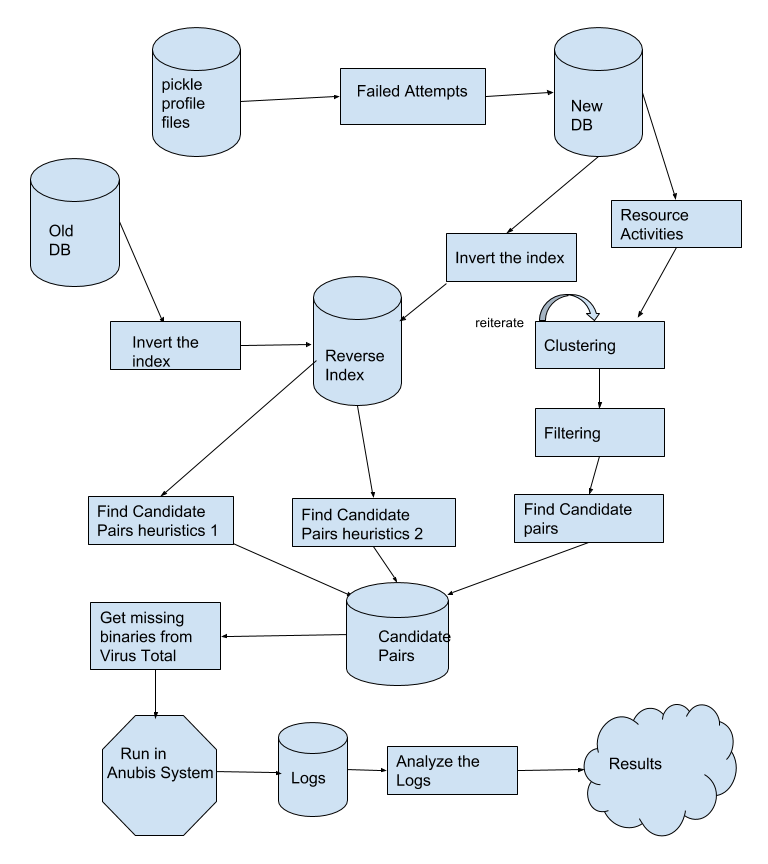
\includegraphics[scale=0.5]{figures/bigpicture.png}
  \caption[Big Picture]{Overview of the research and experiment}\label{fig:bigpicture}
\end{figure}
\section{Summary}
\label{sec:Summary}
In this chapter, we described different terms used in our work in details and also gave an overview of our work flow.
In next chapter, we will show how we implemented the work flow in our system.

%!TEX root = ../main.tex
\chapter{Implementation}\label{chapter:implementation}
In this chapter we give a detail explanation of how we implemented and conducted our research as described in~\autoref{chapter:methodology}.
We start with study of old database structure and creation of reverse index in~\autoref{sec:Old Database and Reverse Index}.
We describe the implementation of the \emph{packer} and the \emph{unpacker} to run the candidate pair inside \emph{Anubis} in~\autoref{sec:packerunpacker} and in~\autoref{sec:Initial Experiment} we run our preliminary test of candidate pairs.
Because the old database did not had record of failed activities, we create the new database with both success and failed resource activity in~\autoref{sec:Creation of Database}.
The implementation of LDA based on resource activities from the newly created database is describe in~\autoref{sec:Document Clustering}.
Finally, in~\autoref{sec:Finding Optimal Candidate Pairs}, we describe the use of max-flow approach and heuristics to find the optimal sets of candidate malware pairs corresponding to interesting resource.

\section{Old Database and Reverse Index}
\label{sec:Old Database and Reverse Index}
Our work was based on wide variety of millions of malware samples, collected over the years, by \emph{Anubis}.
% Our main resource for the research was the direct access of the millions of malware samples from Anubis collected over the years in wild.
We had to effectively and efficiently analyze those to find the behavioral interference between malware families.\\
We started with studying the Anubis system and its database.
We primarily dealt with two database of Anubis backend, the \textbf{`db\_report'} and \textbf{'web\_analysis'}.
The \emph{`web\_analysis'} database was hit first for any binary submitted for analysis from public web interface.
Some of the important tables to our work were \emph{`result', `file', and `file\_task'}.
Each submission is a unique row data in \emph{`result'} table.
A new row is also created in \emph{`file'} table with the \emph{`md5'} and \emph{`sha'} hash of the submitted binary.
We refer the unique primary key of the \emph{`file'} table as \textbf{malware id}.
The \emph{file} and \emph{`result'} tables are associated through \emph{`file\_task'} table.
The analysis of the sample would be done for different behavioral activities related to resources such as File, Registry and Mutex activities.
These activities were saved in `\emph{db\_report}' database.
The resource activities of the malware in \textbf{`db\_report'} database was associated with the \textbf{`web\_analysis'} database by the constraint key \textit{`result\_id'} of the \emph{`result'} table.
In~\autoref{lst:resultidsql}, in the first line, we show a simple \emph{sql} statement to the \emph{result\_id} and \emph{md5} of the binaries submitted to Anubis from the \emph{`web\_analysis'} database.
In the second line, we get the names of the files created by the binary whose \emph{result\_id} is `\emph{12345}' from the \emph{`db\_report'} database.\\
\begin{lstlisting}[language=sql,caption={sql showing database structure to get file created activities of a malware sample},label={lst:resultidsql}]
SELECT result_id, md5 FROM web_analysis.result join web_analysis.file_task using (task_id) join web_analysis.file using (file_id) WHERE task_id = result_id;
SELECT name from db_report.file_created join db_report.file_name using (file_name_id) where result_id = '12345';
\end{lstlisting}

The total number of malware samples that we had in our test database were \textbf{\gettotalmalwarei{}}.
Initially we considered 3 resource types \textit{File, Registry, Mutex}, and queried the database for \textit{create, read, delete} resource activities.
For each resource type, their \textit{create, read, delete} resource activities were queried.
Our first step was to create a reverse index from the database so that we could get the list of malware that created/deleted/read the resource.
Since, the number of malware to process were in millions, trying to save all their activities in a data structure would cause our machine to run out of memory and crash.
We approached this problem with map reduce technique.\\

We worked on a batch of $50,000$ malware at a time, and saved the reverse index of activity to the file with a numbering for each batch.
The resultant numbered files were in the format where resource name and list of unique malware ids were separated by commas (,) as delimiter.
The numbered files of each resource types were sorted, and then joined, to get the final reverse index.
The sort and join operation is shown in~\autoref{lst:sortandjoin} and was fast as it was a merge sort $O( n \times \log(n))$.
Comma is the field separator for both commands and was done on first field which is the resource name.\\

\begin{lstlisting}[numbers=none,language=bash,caption={Sort and join the reverse index},label={lst:sortandjoin}]
  LANG=en_EN sort -t, -k 1,1 $file_name
  LANG=en_EN join -t , -a1 -a2 $file_name1 $file_name2
\end{lstlisting}
A snippet of reverse index of file created activity is shown in~\autoref{lst:reverseindex}, where resource type \emph{`file'}, with resource name \emph{`mbr.exe`}, is created by malware with ids \emph{189524063, 184501719, 87504631, and 86763863}.
\begin{lstlisting}[numbers=none,caption={Sample of reverse index created for File activity},label={lst:reverseindex}]
C:\mbr.exe,189524063,184501719,87504631,86763863
Buttons,111448211
C:/DOCUME~1/ADMINI~1/LOCALS~1/Temp/telnet.exe,178046895,174206059,183601891,89650247
C:/DOCUME~1/ADMINI~1/LOCALS~1/Temp/1.jpg,161552035,116241803
\end{lstlisting}

From the reverse index of the resource activities of the Malware, we mapped created activities against the deleted or read activities.
% We made a list of malware based on the common resource name as the key, where a list of malware which created the resource and another list of malware which delete/read the same resource.
We started looking for one to one interaction of malware to a single resource.
We looked for a set $(a, b)$, where malware `a' creates the resource \emph{r}, and malware `b' deletes the same resource, \emph{r}, such that no other malware has create or delete activities on that resource \emph{r}. We ran those malware pairs in the Anubis system using the \emph{Unpacker}.
\section{Packer and Unpacker}
\label{sec:packerunpacker}
In order to run the pair of malware together inside the Anubis environment we made a Win32 console application (Anubis VM is based on Windows OS.\@), named \textbf{Unpacker}.
We used the fact that we can append any data at the end of Windows PE executable, and it would not affect the executable's program flow.
We wrote a \textbf{packer} program that would add the candidate binary pair at the end of the \emph{Unpacker} binary and then further appends the time delay and file size of each candidate binary as meta information.
The structure of the Unpacker binary is shown in~\autoref{fig:unpacker}.
The \emph{Unpacker} binary, when executed, would read itself from the back to get the meta information and read candidate binaries bytes.
% We created a meta binary, that will read itself, and extract the other two binaries, that will be attached to it.
It will then create the candidate binaries from the read bytes, and run both binaries with a time delay given.\\
\begin{figure}[htbp]
  \centering
  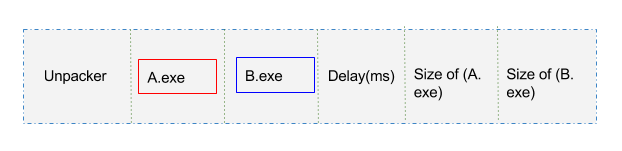
\includegraphics[scale=0.5]{figures/unpacker.png}
\caption{Structure of the Unpacker binary that would create the candidate pair and run them with delay.}
\label{fig:unpacker}
\end{figure}

Code snippet of the \emph{`Unpacker'} binary is shown in~\autoref{lst:unpacker.c}.
We used a struct of 3 integer size to read and hold the meta information. The size of last three \textit{unsigned int} byte of \emph{Unpacker} has the binary pair sizes information and the delay time, known as meta information.
The offset for meta-information was calculated by deduction of $3 \times \textit{size of `uint'}$ from the total size of itself (Unpacker).
We calculate the starting position of appended binaries, and use \texttt{`fseek\(\)'} function to set the file position pointer there.
We then start reading the bytes until the exact size of binary is read.
The read bytes were then saved to create new binary file.
We used \emph{windows.h} standard library's functions: \emph{`CreateProcess'} function to execute the binary, and \emph{`Sleep'} function for delay in between two execution.\\

\begin{lstlisting}[language=c,caption={snippet of Unpacker.c file}, label={lst:unpacker.c}]
  /* stuct for storing meta information */
  typedef struct {
    unsigned int delay;
    unsigned int fsize1;
    unsigned int fsize2;
  }meta_info;

  /* reading the meta information and first binary */
  rfp = fopen(argv[0], "rb");
  wfp1 = fopen(fileName1, "wb");

  fseek(rfp,0,SEEK_END);
  size = ftell(rfp);
  offset = size - sizeof(meta_info);
  fseek(rfp, offset, SEEK_SET);
  fread(&info, 1, sizeof(info), rfp);

  /* calculate the unpackersize from the offset and files size. */
  unpackersize = offset - (info.fsize1 + info.fsize2);

  /* rewind back and to the point of the start of file1 */
  fseek(rfp,0,SEEK_SET);
  fseek(rfp, unpackersize, SEEK_SET);

  nread_sofar = 0;
  while (nread_sofar < info.fsize1) {
      nread = fread(buf, 1, min(info.fsize1 - nread_sofar, sizeof(buf)), rfp);
      nread_sofar += nread;
      fwrite(buf, 1, nread, wfp1);
  }
  fclose(wfp1);
 \end{lstlisting}
\section{Initial Experiment}
\label{sec:Initial Experiment}
During our initial run of candidate pairs, we found lots of dropper malware causing this interaction.
For a candidate pair $(a,b)$, binary `a' was a dropper that would create many binaries including the binary `b', and binary `b' actually read itself upon execution, which was recorded as read activity by Anubis.
After running many other candidate pairs and analyzing the results manually, we were able to understand the Anubis report in depth and also found a logical error on our current approach.\\

Our notion behind checking the malware interaction was finding candidate pairs such that one malware `a' creates some resource, `r', and another malware `b' tries to access or delete the same resource, `r'.
But, Anubis ran each submitted binaries in an isolated environment; hence there was no way that a malware sample `b' would find the resource that was supposed to be created by malware `a'.
We should have been looking for failed attempt activities, where a malware sample unsuccessfully tries to access or delete a resource created by another malware.
But, the current database had no record of such failed attempt.
This lead us to look for the alternatives where we could find log of such failed attempt activities during the execution of binary.\\

We parsed the behavioral profiles, as described in~\autoref{sub:Behavioral Profile}, of malware samples to find failed activities of deletion and access.
\section{Creation of Database}
\label{sec:Creation of Database}
Recreating the database was one of the bottleneck in our project and consumed much time.
The behavioral profile files had to be accessed via network file system.
We need to walk through large list of directories and file, to find the behavioral profile pickle~\cite[]{pythonpickle} of specific malware.
We found \emph{\gettotalmalwareii{}} behavioral profile files out of \emph{\gettotalmalwarei{}} malware.\\

We considered eight resource type into account while parsing the profile files: File, Registry, Sync, Section, Process, Service, Job, and Driver [see \autoref{sub:Resource Types and Activities}].
Windows Native and Windows API calls were generalized into OS Operation during the creation of behavioral profile.[see~\autoref{sub:Behavioral Profile}]
We went through the list of OS Operations~[\autoref{ssub:OS Operations}] and mapped them into the broad three categories \emph{Modify, Access, and Delete}.
The modify, access, and read list for the resource types \emph{\getresourcetypes{}} are shown in~\autoref{lbl:ntapi}.


\begin{lstlisting}[numbers=none,language=ruby,caption={Mapping of generalized OS Operation from behavioral profile},label={lbl:ntapi}]
MODIFY_LIST = {
        file:      ["create_named_pipe", "create_mailslot", "create", "rename", "set_information", "write", "flush_buffer", "map"],
        registry:  ["create", "restore_key", "save_key", "set_value", "set_information", "mem_write"],
        process:   ["create", "set_information", "suspend", "resume", "unmap", "map"],
        job:       ["assign", "set_information"],
        driver:    ["unload", "load"],
        section:   ["create", "map", "unmap", "mem_write", "set_information"],
        sync:      ["create", "map", "set_information", "mem_write"],
        service:   ["create", "start", "control"]
        }

ACCESS_LIST = {
        file:      ["query_file", "query", "open", "query_directory", "query_information", "read", "monitor_dir", "query_value"],
        registry:  ["enumerate", "enumerate_value", "monitor_key", "open", "query", "query_value", "mem_read"],
        process:   ["open", "query"],
        job:       ["open", "query"],
        driver:    ["query"],
        section:   ["open", "query", "mem_read", "read", "query_file", "query_system"],
        sync:      ["open", "query"],
        service:   ["open"]
        }

DELETE_LIST = {
        file:      ["delete", "open_truncate"],
        registry:  ["delete", "delete_value"],
        process:   ["delete"],
        job:       ["delete"],
        driver:    ["delete"],
        section:   ["delete"],
        sync:      ["delete"],
        service:   ["delete"]
        }

\end{lstlisting}

Each malware submitted to Anubis had its own unique behavioral profile saved as python pickle~\cite{pythonpickle} object.
We parsed behavioral profile and extracted the object names and operations from the \emph{OS Object} and \emph{OS Operations} respectively.
The object name is the name of the resource and operations is the activity performed on the resource.
The OS operation was categorized into \emph{modify}, \emph{access}, and \emph{delete} activity according to the mapping in~\autoref{lbl:ntapi}.
The status of the operation, failed or successful, was also taken into account this time.
With the resource name, operations and status, we create a new database of malware activities.

We used \textbf{MySql Version 5.5.46} as our database engine. MySQL~\cite[]{mysql} is highly scalable and flexible relational database system which complies with the ACID model~\cite[]{acid} design principle.
We used multiple workers to create the database, and ACID compliance prevented from inconsistency of data when being updated across multiple tables.\\

% The basic CRUD operations were time expensive and made the overall operation slow.
While creating the new database, we hit the integer overflow for the primary index key of `\emph{registry access}' table.
We did not anticipate the number of records to cross maximum \emph{`int (10)'} limit \emph{4,294,967,295}.
We created another ``\emph{registry access}' table, with different table name, and start inserting the registry access records in the new table.
When accessing the data for later, we re-factored our program so that we checked both the registry tables in order to find the registry access activities of a malware sample.
The final database size was 1.2 Terabyte.\\
% We performed database tuning (buffer size, query cache, threads pool) to increase the speed of database operations.
% We used \emph{cPickle}, which made the reading of pickle file 3 times faster than default python \emph{pickle} module.

We processed \gettotalmalwareii{} behavioral profiles.
About $62\%$ of execution time was taken to load the gzip pickle~\cite[]{pythonpickle} of malware profile and the normal SQL CRUD (create, read, update, and delete) operation, which can be seen in Figure~\ref{fig:dbcreation}.
% The execution profile is shown in~\autoref{fig:dbcreation}
%TODO: put profile.png
\begin{figure}[ht]
    \centering
    \def\svgwidth{\columnwidth}
    \scalebox{0.99}{\input{figures/dbcreate.pdf_tex}}
    % \input{figures/overview.pdf_tex}
\caption{Profile of new database creation}
\label{fig:dbcreation}
\end{figure}

After the creation of new database, we made a reverse index, like before, for the `\emph{resource name}' to `\emph{malware ids}' modifying, accessing, and deleting the resource.
This time the refined database had both the success and failed resource activities.
% Getting all the resource activities related to all the resource types \emph{file, registry, section, driver, sync,service, process, and job} was also time expensive.
The reverse indexes were used to map resources that were successfully modified with resources that were read/accessed with failed attempt.
For instance, we made a mapping between file successfully modified and failed file deletion, and mapping between file successfully modified and failed file access.
We made same mapping for all other 7 resource types.
All the mapping was done based on the common `\emph{resource name}'.\\

With the reverse index mapping, we chose the candidate pairs such that one malware created the resource and another malware made a failed attempt to delete/access the same resource.
But, the number of possible pairs were too many with this simple heuristic and we hit the \emph{n-combination} problem.
A single resource \texttt{`r'} would have been created by tens of thousands of malware and another tens of thousands of malware trying to access/delete it unsuccessfully.
The combination of candidate pairs from the candidate sets with thousands of malware are of large number to run and analyze result.\\
%TODO: add one more reason "not good enough"

We wanted to filter our candidate sets without compromising the quality.
We performed clustering of the malware based on their resource activities (behavior) to address this problem.
Malware dataset were clustered into different families and candidate pairs were chosen such that they belong to different families.
\section{Document Clustering}
\label{sec:Document Clustering}
We filtered our malware dataset from the reverse index mapping by removing all resource activity that we confirmed as benign based on our knowledge.
We sorted the reverse index (resource name to malware ids) with respect to the number of malware ids associated with the resource name in descending order.
With this, we had most commonly modified/accessed/created resource at the top of the list.
We went through the resource name until we found some interesting resource name which does not look benign.
We excluded all benign resources preceding the first interesting suspicious resource name.
For instance, file resource name such as \emph{`Dr.\ Watson.exe'} and \emph{`Sample.exe'} were some resources with highest number of malware interacting with them.
The reasons are \emph{`Dr Watson'} file is created whenever a binary crashes and \emph{Sample.exe} is the name, the submitted binary gets renamed to, by Anubis.
We filtered all such benign resource activities related to resource type file, registry, section, sync, and process.
Resource types service, job, and driver did not have any interesting mapping.
The total number of malware samples were filtered to {\gettotalmalwareiii{}}.\\

We created the text corpora for those {\gettotalmalwareiii{}} malware, and performed the document clustering.
We converted all the resource activities related of the malware samples into the corpora text as discussed in~\autoref{sub:Clustering}.
Each resource activity was represented as word, each malware was represented as the document, and the collection of documents were text corpora.
The process was database intensive as seen in Figure~\ref{fig:actcreation}, and took almost week for us to get complete text copora.
The resultant text corpora was about 81 Gigabytes of data.
% After days of running the script, we could gather all the resource activity of {\gettotalmalwareii} malware as the corpus for algorithm.
\begin{figure}[ht]
    \centering
    \def\svgwidth{\columnwidth}
    \scalebox{1}{\input{figures/activities_creation.pdf_tex}}
    % \input{figures/overview.pdf_tex}
\caption{Profiling of building a corpus}
\label{fig:actcreation}
\end{figure}
% \begin{figure}
% \begin{center}
%   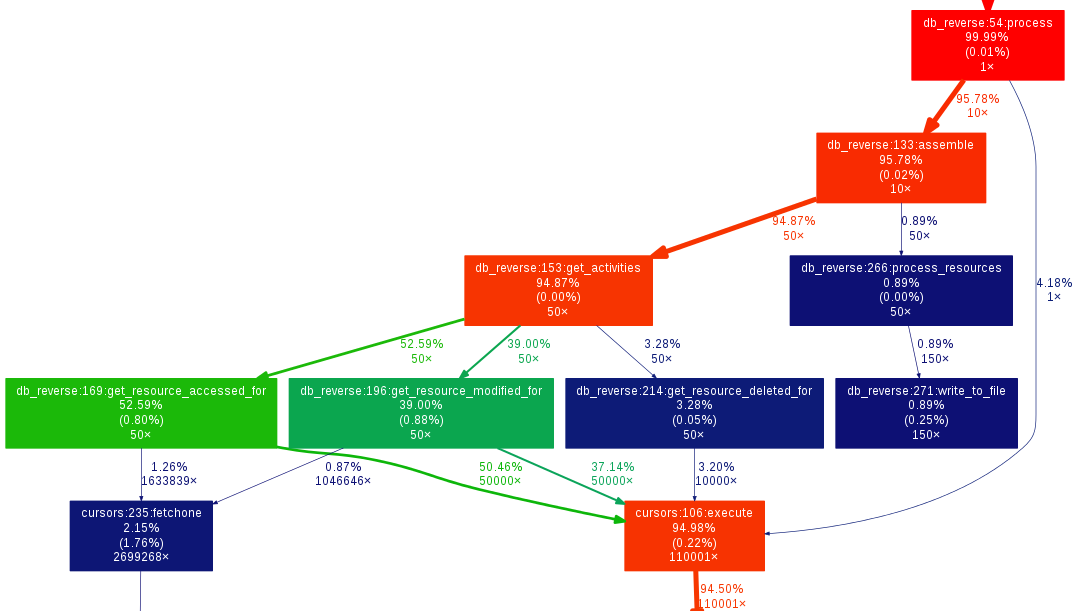
\includegraphics[scale=0.4]{figures/activities_creation.png}
% \end{center}
% \end{figure}
\\
\subsection{LDA Model}
\label{sub:LDA Model}
We used python module Gensim~\cite[Gensim]{gensim}  for the clustering and used the LDA multicore model which we described in~\autoref{ssub:Gensim}.
The LDA model generation code snippet is show in~\autoref{lst:lda.py}.
The corpora consisted of one document per line.
We created a dictionary from the corpora using Gensim \emph{`corpora.Ditionary`} module~\cite[]{gensimdict}.
Dictionary is representation of all the unique tokens (words) by a unique token-ids.
We filtered the dictionary by discarding any resource activity that occurred in less than 10 or more than 1 million for clustering, as those activities are too less or too common to take into consideration.
% The lower and upper limit were chosen based the cumulative distribution function graph of resource activities.
We kept only $200,000$ tokens after the filtering.
This is done in line $7$~[\autoref{lst:lda.py}], where the arguments passed into \emph{`filter\_extremes'} method are minimum threshold (which is 1000), maximum threshold in fraction (which is $0.14$: 1,000,000 out of total \gettotalmalwareiii{} documents), and total number of frequent words to keep after filtering (which is $200,000$).
In line 9--12~[\autoref{lst:lda.py}], we make an iterator to read the corpus.
The iterator operates on each line, which represents a document, of corpus text file and yields a bag of words of the document.
Bag of words is a list of two-element tuple, which represents word (token-id) and its count (number of occurrence) in document.
In line 15~[\autoref{lst:lda.py}], we create a LDA model for our corpus with 1000 topics.
The LDA gives the probability of different clusters that a document can belong to and we assign the document to the cluster with highest probability.\\
% The malware samples were clustered into 752 unique topics.
% This was based on heuristic after studying the cdf graph of activities to number of malware.
%TODO: add cdf of reverse index
% The number of topic was chosen to be 1000, however our malware samples were distributed among only 752 unique topic.
\begin{lstlisting}[float,floatplacement=H,language=python,caption={Script to run Gensim LDA},label={lst:lda.py}]
from gensim import corpora, models
import sys
document_name = sys.argv[1]
# read the file with malware activities and create dictionary
dictionary = corpora.Dictionary(line.split() for line in open(document_name))
# filter the dictionary for extreme
dictionary.filter_extremes(no_below=10,no_above=0.14,keep_n=1000000)
# create a iterator corpus as the file is large 80GB
class MyCorpus(object):
    def __iter__(self):
        for line in open(document_name):
            yield dictionary.doc2bow(line.split())

corpus = MyCorpus()
lda = models.ldamulticore.LdaMulticore(corpus=corpus,id2word=dictionary,num_topics=1000)
\end{lstlisting}

The number of clusters created were \textbf{``662''}.
The largest cluster size was {\getlargestclustersize{}} and the lowest was {\getlowestclustersize{}}.
The histogram and cumulative distributive graph showing the sizes of cluster can be seen in~\ref{fig:histclustersize},~\ref{fig:ecdfclustersize}, and~\ref{fig:cdfclusterlen}.
From the graph we can see that distribution of cluster size was mostly below 50,000.
$90\%$ of the cluster, about \emph{629 out of 662}, falls under the cluster size of less than 50,000.
Similarly, \emph{4 million} malware, which is the $65\%$ of total malware clustered, are in the cluster size of less than 50,000.\\
\begin{figure}[htbp]
\begin{center}
  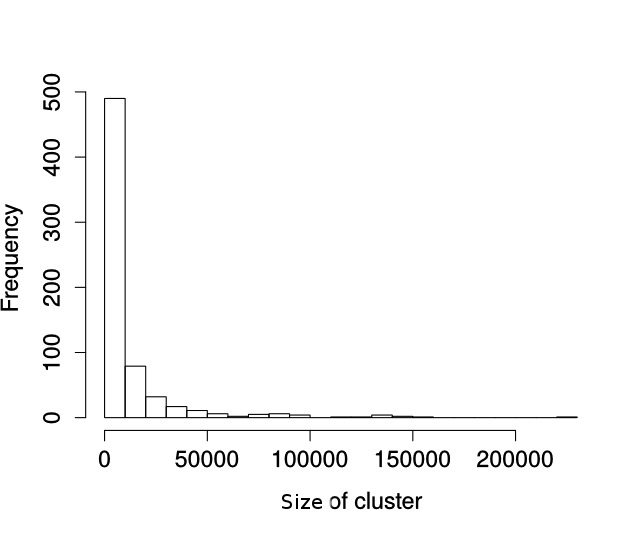
\includegraphics[scale=0.5]{figures/histclustersize_new.png}
\end{center}
\caption{Histogram showing the distribution of Cluster size}
\label{fig:histclustersize}
\end{figure}
\begin{figure}[htbp]
\begin{center}
  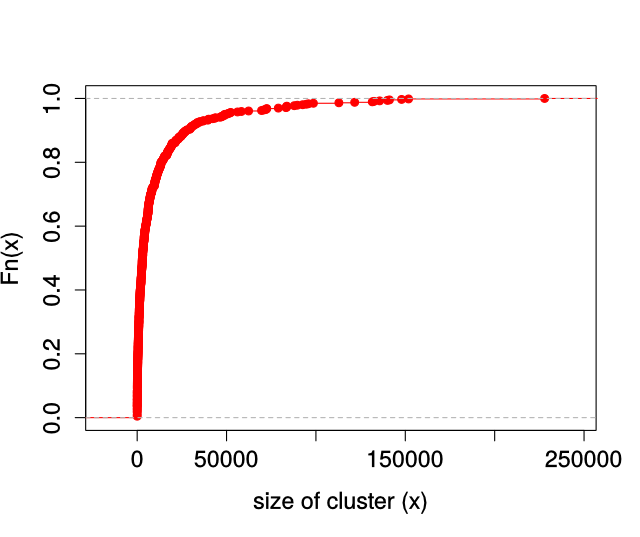
\includegraphics[scale=0.5]{figures/ecdfclustersize.png}
\end{center}
\caption{CDF between size of cluster and topic fraction}
\label{fig:ecdfclustersize}
\end{figure}
\begin{figure}[htbp]
\begin{center}
  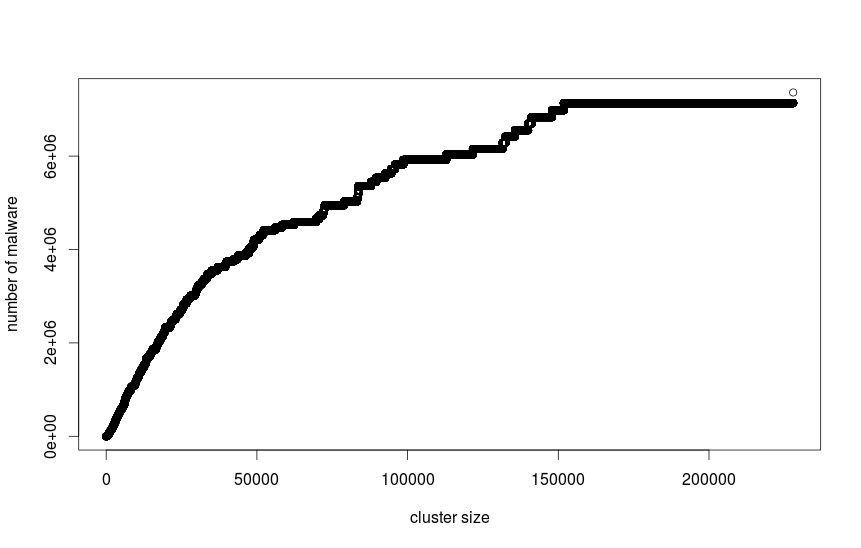
\includegraphics[scale=0.3]{figures/cdfclusterlen2.png}
\end{center}
\caption{CDF between size of cluster and total number of malware}
\label{fig:cdfclusterlen}
\end{figure}
\subsection{Inter-Distance and Intra-Distance}
\label{sub:Inter-Distance and Intra-Distance}
We calculated the distance based on the average number of common words between the malware pair.
\textbf{Intra-distance} represents the average number of common words between the malware pair from same cluster.
\textbf{Inter-distance} represents the average number of common words between the malware pair from different clusters.
Since we want to cluster malware with similar behavioral activity together in same cluster; the intra-distance should be high (higher similarity among malware samples of same cluster), and the inter-distance should be low (lower similarity among malware samples from different cluster).
\\

To show the quality of our clustering we provide the following graph showing the graph of inter-cluster and intra-cluster distance in Figure~\ref{fig:intraclustcommon} and Figure~\ref{fig:interclustcommon}.\\
In case of intra-distance, for a cluster, we randomly selected 1000 malware pair (if possible because there were some clusters of size as small as 1), from the combinations of malware samples belonging to that cluster.
We calculated the average number of common resource activities\textit{(words)} present among the malware\textit{(document)} pair.
We can see that the average common words between the intra malware sample were good with intra-distance of at least \emph{500} covering $80\%$ of family topics~[\autoref{fig:intraclustcommon}].
For the inter-distance calculation, a cluster was paired with other clusters, and from those cluster pair,
we randomly selected 1000 malware pair (if possible because there were some clusters of size as small as 1).
We calculated the average common resource activities between those malware pairs to get the inter-distance.
We can see that the inter-distance of only 10 was covering almost $90\%$ of family topic~[\autoref{fig:interclustcommon}].
\begin{figure}[htbp]
\begin{center}
  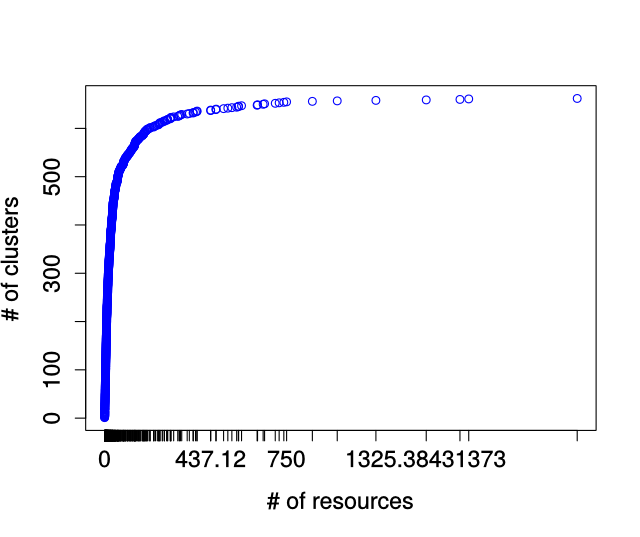
\includegraphics[scale=0.7]{figures/intra_clustered_common.png}
\end{center}
\captionsetup{font=small}
\caption{ Graph showing cdf distribution of common resource between same family topic}
\label{fig:intraclustcommon}
\end{figure}
\begin{figure}[htbp]
\begin{center}
  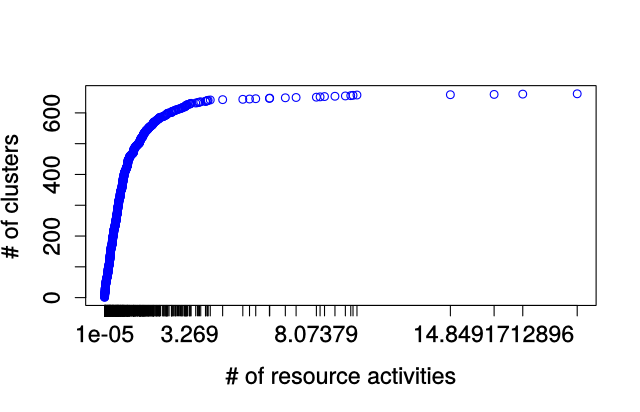
\includegraphics[scale=0.7]{figures/inter_clustered_common.png}
\end{center}
\captionsetup{font=small}
\caption{Graph showing cdf distribution of common resource between different family topic}
\label{fig:interclustcommon}
\end{figure}

\section{Finding Optimal Candidate Pairs}
\label{sec:Finding Optimal Candidate Pairs}
After the clustering, tens of thousands of malware associated with the resource, would now be reduced and represented by hundreds of families (clusters), that those malware belong to.
As described in~\autoref{sub:Candidate Selection}, we chose the candidate pair corresponding to a resource, such that each malware in the pair belongs to different clusters.
% We need to make sure that the family pair associated with the single resource is not repeated.
% We needed to further filter the candidate pairs, such that malware pair from same clusters, does not repeat for different resource name.
In order to find the optimal set of candidate pairs we interpreted the interaction of malware and resource, with respect to cluster, into Flow Network.
\subsection{Max Flow Approach}
\label{sub:Max Flow Approach}
We wanted to find the optimal pair of malware such that we have all the interesting mapped resource covered along with the cluster associated with it.
We represented the mapping between the resource, malware, and cluster as a flow network, and run the max flow algorithm as given in Figure~\ref{fig:maxflow}.\\

The network is made of 4 layers, other than sink and source.
Layer one is read/delete malware, the malware samples that tried to access or delete interesting resources but failed.
Layer two is combinations of clusters (\emph{ic=input-cluster}), that the malware with failed access or delete attempt belongs to, and the resource on which the malware tried to operate.
Layer three is the combinations of clusters (\emph{oc=output-cluster}), that the malware with successful modification operation belongs to, and the resource that they could successfully modify.
Layer four is the malware that successfully modified the resource.\\
The flow rules were:
\begin{itemize}
  \item All malware from layer one is connected from sources and also connected to the input cluster and resource combination it belongs to.
  \item All input-cluster and resource combination in layer two is connected to all output cluster resource combination in layer 3 that has a matching resource.
  \item All output-cluster and resource combination in layer 3 is connected to the corresponding malware in layer 4.
  \item Each malware in layer 4 is connected to the sink (T).
\end{itemize}
The capacities were:
\begin{itemize}
  \item All connections have capacity of infinite except connections from layer 2 to layer 3.
  \item All connections from layer 2 to layer 3 have a capacity of one.
\end{itemize}

\begin{figure}[htbp]
  \centering
  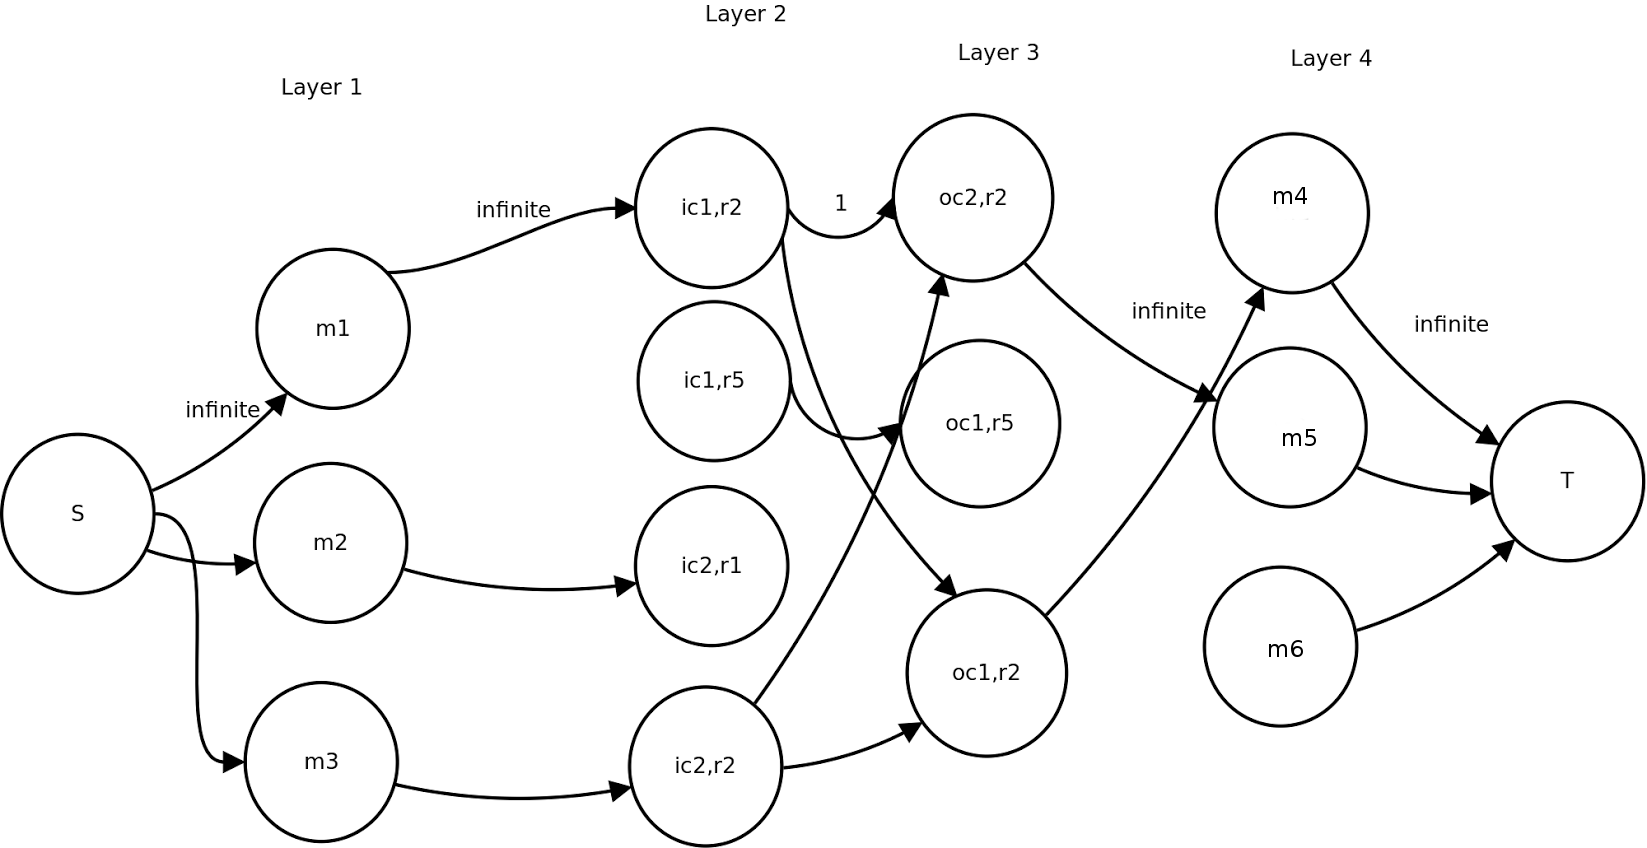
\includegraphics[scale=0.23]{figures/maxflow2.png}
  \caption[Max Flow]{Graph representing the max flow implementation}\label{fig:maxflow}
\end{figure}

The maximum flow in this network corresponds to an optimum match up.
To explain, in~\autoref{fig:maxflow}, `$m_1$' in layer 1 is connected to $(ic_1,r_2)$ in layer 2.
There are two cluster-resource combination, $(oc_2,r_2)$ and $(oc_1,r_2)$, in layer 3, that has resource `$r_2$' common with $(ic_1,r_2)$ cluster-resource combination.
So our candidate pairs would be, $(m_1,m_5)$ and $(m_1,m_4)$ operating on $r_2$'.
Path from source (S) to $m_2$ in layer 1 and $(ic_2,r_1)$ which does not reach the sink (T), thus, is omitted.
%TODO: maxflow did not provide optimal
% The max flow approach, did lower
The max flow approach gave us optimal candidate pairs such that each pair of cluster is only covered once.
However, the approach did not take care of repetition of cluster pair corresponding to different resource.
% If malware pair $(m_1,m_2$) is associated with resource $(r_1,r_2,r_3)$, same candidate pairs gets repeated three times.
If malware $m_1$ is belongs to input cluster $ic_1$ and malware $m_2$ belongs to output cluster $oc_2$ and both are associated with resource $(r_1,r_2,r_3)$, same candidate pairs $(m_1,m_2)$, belonging to same cluster pair $(ic_1,oc_2)$, gets repeated three times.
% We wanted to group those repetition so that we get only single candidate pair $(m_1,m_2)$and analyze the behavioral interference they might have on different resources.
We wanted to group those repetition so that we get single candidate pair $(m_1,m_2)$ that covers the unique cluster pair $(ic_1,oc_2)$, for all its corresponding resources $(r_1,r_2,\ldots)$.
We used heuristics approach to eliminate those repetition.
\subsection{Heuristics Approach}
\label{sub:Heuristics Approach}
% We see in the first approach, we are not covering all resource interactions that were meticulously carved from millions of data points. 
The problem was to find the ``minimal set'' of malware pairs that covers all unique cluster (family) pairs (dictated by the set of all candidate pairs) and it also covers all resources that help build the candidate pairs, i.e., for each resource \emph{`r'} from resources \emph{`R'}, at least one malware pair from the final set should correspond the resource \emph{r}.\\

The relations has been represented in the graph below, where, \emph{I} is a set of input clusters from set \emph{`A'} and \emph{`O'} is the set of output clusters from set \emph{`B'}.
Set \emph{`A', `B'} are the sets of malware samples successfully modifying the resource and accessing/deleting the resource with failed attempt, respectively.
\emph{`R'} is the set of all interesting resources.
% They have also been described in the\textit{~\autoref{sub:Candidate Selection}}.
\begin{figure}[htbp]
  \centering
  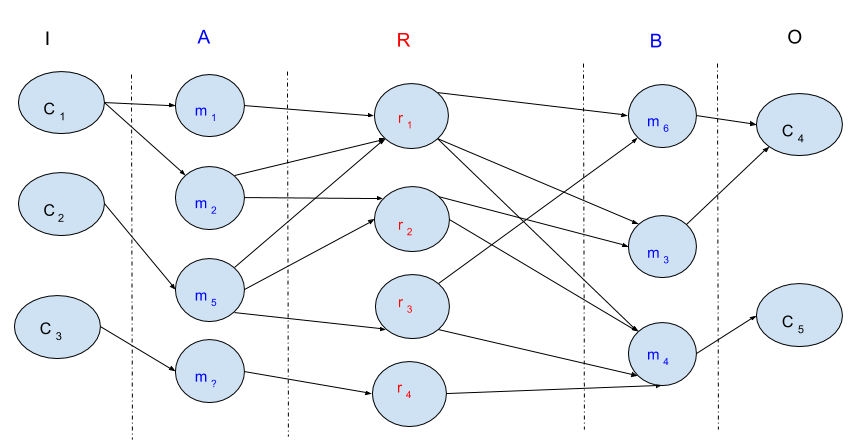
\includegraphics[scale=0.45]{figures/dhkheuristics.png}
  \caption[]{Heuristics approach to optimal malware pair selection}\label{fig:dhkheuristics}
\end{figure}
\\

In the Figure~\ref{fig:dhkheuristics},  $m_1,m_2, m_5$ samples create resource $r_1$, which is accessed (failed attempt) by $m_6, m_3$, and $m_4$.
The malware $m_1$ and $m_2$ maps to cluster $c_1$. Malware $m_6$ and $m_3$ maps to cluster $c_4$, and so on.
We need to find the minimal number of paths from each element \emph{$c_x$} of set \emph{`I'} to all reachable elements in \emph{`O'} (reachable from \emph{$c_x$}), such that all reachable elements \emph{`r'} in \emph{`R'} (reachable from \emph{$c_x$}) are traversed.
From such minimal set, we generated the candidate pairs by taking members of \emph{A} and \emph{B} from the path.
% This should work as we hard clusters (sample only falls into one cluster).
\\

We created the data structure as shown in~\ref{lst:dbdict}.
The data is a dictionary.
All candidate cluster pairs are keys and the value is a dictionary whose keys are malware pairs (all candidate malware pairs belonging to the cluster pair) and values are the list of corresponding resource.
\begin{lstlisting}[language=python,floatplacement=htpb,caption={Database Structure},label={lst:dbdict}]
db = { (c_i, c_o) :
    { (m_a, m_b) : [ r1, r2 ,...],
        ...,
     }
}
\end{lstlisting}
\begin{lstlisting}[float,floatplacement=htbp,language=python,caption={Pseudo code (Python) to get minimal set of candidates for all resource},label={lst:heuristicalgo}]
candidate_set = set()
for c_pair, v in db.iteritems():
    # reverse sort malware pairs by number of associated resources
    x = sorted( [(len(b), a) for a,b in v.iteritems()] , reverse=True)
    r_set = set()
    for c, m_pair in x:
        cur_r = v[m_pair]
        if not r_set.issuperset(cur_r):
            r_set = r_set.union(cur_r)
            candidate_set.add(m_pair)
\end{lstlisting}

The reduced candidate set was computed as shown in pseudo-code~\ref{lst:heuristicalgo}.
It is a greedy algorithm starting from the malware pair that corresponds most number of resource interactions.
For each malware pair it checks if that pair has been already chosen, and if not, adds the pair to the candidate list.
% \section{Testing the Candidate Pairs}
% \label{sec:Testing the Candidate Pairs}

%!TEX root = ../main.tex
\chapter{Results}\label{chapter:results}


% %!TEX root = ../main.tex
\chapter{Future Work}\label{chapter:future_work}
%!TEX root = ../main.tex
\chapter{Conclusion and Future Work}\label{chapter:conclusion_and_future_work}

% TODO: add more chapters here

\appendix{}

 % TODO: remove if glossary not needed
\glsaddall{} % add all defined terms to glossary, even if not referenced in text
\printglossaries{}

\microtypesetup{protrusion=false}
\listoffigures{}
\listoftables{}
\microtypesetup{protrusion=true}
\printbibliography{}

\end{document}
